\chapter{Rachunek prawdopodobieństwa}

Materiały teoretyczne zostały opracowane na podstawie \href{https://drive.google.com/file/d/1WlyT05bbN8DMYJ59sRA7HeTXgpvc7yQ4/view}{notatek Błażeja Wilkoławskiego}, \href{https://wazniak.mimuw.edu.pl/index.php?title=Rachunek_prawdopodobie%C5%84stwa_i_statystyka}{materiałów na Ważniaku} oraz \href{https://www.mimuw.edu.pl/~ados/MNRP/MNRP.pdf}{skryptu z Metodyki Nauczania Rachunku Prawdopodobieństwa autorstwa Adama Osękowskiego}.

\section*{Podstawa programowa}
\begin{enumerate}
    \item \textbf{Prawdopodobieństwo warunkowe i całkowite}, wzór Bayesa, niezależność zdarzeń.
    \item \textbf{Dyskretne zmienne losowe} i ich rozkłady: dwumianowy, geometryczny, Poissona.
    \item \textbf{Parametry rozkładu}: wartość oczekiwana, wariancja, funkcje tworzące prawdopodobieństwa.
    \item \textbf{Nierówności probabilistyczne}: Markowa, Czebyszewa, Chernoffa.
    \item \textbf{Ciągłe zmienne losowe}: definicja, własności, rozkład wykładniczy oraz normalny, centralne twierdzenie graniczne.
    \item \textbf{Łańcuchy Markowa}: prawdopodobieństwa oraz średnie czasy dotarcia, twierdzenie ergodyczne.
    \item \textbf{Wnioskowanie statystyczne}: estymatory nieobciążone, estymatory największej wiarygodności.
\end{enumerate}

\section{Prawdopodobieństwo warunkowe i całkowite}

\textbf{Doświadczeniem losowym} nazwiemy dowolny proces bądź ciąg czynności taki, że:
\begin{itemize}
    \item jego sposób wykonania i warunki są ściśle określone, a sam proces można dowolnie wiele razy powtarzać,
    \item zbiór możliwych wyników procesu (\textbf{zdarzeń elementarnych}) jest z góry znany,
    \item wyniku konkretnego doświadczenia nie można z góry przewidzieć.
\end{itemize}

Zbiór wszystkich zdarzeń elementarnych oznaczamy wielką literą $\Omega$.

W wielu sytuacjach interesuje nas nie tyle konkretny wynik doświadczenia (pojedyncze zdarzenie elementarne), ale to, czy należy on do wcześniej ustalonego podzbioru wszystkich zdarzeń elementarnych. Takie podzbiory nazywamy \textbf{zdarzeniami} i zwyczajowo oznaczamy wielkimi literami alfabetu, np. $A, B, X, Y...$

\begin{example}
    Dla doświadczenia losowego będącego rzutem kostką, zbiorem zdarzeń elementarnych jest $\Omega = \{1, 2, ..., 6\}$, a przykładowymi zdarzeniami:
    \begin{itemize}
        \item $A = \{2, 4, 6\}$ -- wypadła liczba parzysta
        \item $B = \{1, 2, 3, 4, 5, 6\}$ -- coś wypadło
        \item $C = \pusty$ -- nic nie wypadło
    \end{itemize}
\end{example}

\textit{Uwaga:} ponieważ w programie studiów informatycznych nie zajmujemy się innym prawdopodobieństwem niż prawdopodobieństwo klasyczne, pominiemy tutaj formalizmy związane z przestrzeniami probabilistycznymi -- nie są one potrzebne przy rozwiązywaniu zadań. Zaznaczymy jedynie, że przestrzenie te służą do definiowania sposobu przypisania poszczególnym zdarzeniom ich prawdopodobieństw.

\subsection{Podstawowe własności prawdopodobieństwa}

Niech $\Omega$ będzie niepustym zbiorem wszystkich zdarzeń elementarnych doświadczenia losowego, a $P$ -- prawdopodobieństwem określonym na podzbiorach $\Omega$. Wtedy:
\begin{itemize}
    \item dla każdego zdarzenia $A$ zachodzi $P(A) \in [0, 1]$, przy czym $P(\pusty) = 0$ oraz $P(\Omega) = 1$
    \item dla dowolnych zdarzeń $A, B$, takich że $A \subseteq B$, jest $P(A) \leq P(B)$
    \item $P(A') = 1 - P(A)$, gdzie $A'$ to zdarzenie przeciwne do zdarzenia $A$
    \item dla dowolnych zdarzeń $A, B$ mamy $$P(A \cup B) = P(A) + P(B) - P(A \cap B)$$
\end{itemize}

\begin{wrapfigure}{r}{5cm}
    \vspace{-5mm}
    
    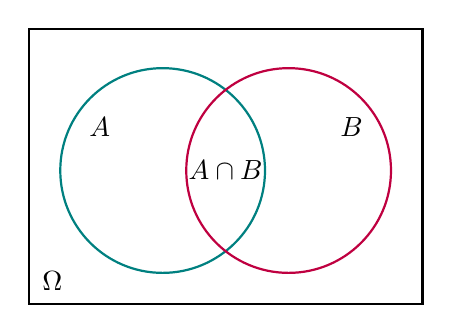
\begin{tikzpicture}
        \draw[black, thick] (-1.5,-1.5) rectangle (3.5,2);
        \draw[teal, thick] (0.2,0.2) circle (1.3);
        \draw[purple, thick] (1.8,0.2) circle (1.3);
    
        % Etykiety
        \node at (-0.6, 0.75) {$\teal{A}$};
        \node at (2.6, 0.75) {$\purple{B}$};
        \node at (-1.2, -1.2) {$\Omega$};
        \node at (1, 0.2) {$A \cap B$};
    \end{tikzpicture}
\end{wrapfigure}

Przydatnym trikiem jest \purple{wizualizacja geometryczna} przestrzeni probabilistycznej za pomocą \textbf{diagramów Venna}, czyli schematów służących ilustrowaniu zależności między zbiorami (w naszym przypadku -- między zdarzeniami).

Z rysunku łatwo odczytać na przykład powyższy wzór na prawdopodobieństwo sumy zdarzeń $P(A \cup B)$ oraz wiele innych nieoczywistych relacji, jak np.
$$P(A' \cup B) = 1 - P(A \setminus B)$$

\subsection{Schemat klasyczny}

Aby móc wygodnie obliczać prawdopodobieństwa interesujących nas zdarzeń, w większości przypadków będziemy sprowadzać całe rozumowanie do problemu kombinatorycznego za pomocą \textbf{schematu klasycznego}.

Załóżmy, że $\Omega$ jest zbiorem skończonym i wszystkie zdarzenia elementarne są jednakowo prawdopodobne. Wówczas dla każdego $\omega \in \Omega$ oraz $A \subseteq \Omega$ zachodzi
$$\purple{P(\omega) = \frac{1}{|\Omega|}} \textqq{oraz} \purple{P(A) = \frac{|A|}{|\Omega|}}$$

\begin{example}
    Obliczymy prawdopodobieństwo, że w losowej 5-kartowej ręce pokerowej jest dokładnie jedna para (w szczególności nie ma w niej żadnej trójki ani dwóch par).
    
    W naszym przypadku $\Omega$ to zbiór wszystkich 5-elementowych podzbiorów 52 kart, mamy więc $|\Omega| = \binom{52}{5}$. Niech $A$ będzie zbiorem wszystkich układów z dokładnie jedną parą. Ponieważ każdy 5-elementowy podzbiór kart jest równie prawdopodobny, korzystamy ze schematu klasycznego i dostajemy $P(A)=\frac{|A|}{|\Omega|}$.
    
    Sprawdźmy, na ile sposobów można wybrać jedną parę:
    \begin{enumerate}
        \item na 13 sposobów wybieramy rangę kart w parze,
        \item na $\binom{4}{2}=6$ sposobów wybieramy kolory tych kart,
        \item na $\binom{12}{3}$ sposobów wybieramy rangi pozostałych kart (muszą być różne),
        \item na $4^3$ sposobów wybieramy kolory tych kart.
    \end{enumerate}
    Ostatecznie $|A|=13\cdot6\cdot\binom{12}{3}\cdot4^3$ oraz $P(A)\approx0,423$. Jak widać, użycie schematu klasycznego sprowadziło problem probabilistyczny do problemu kombinatorycznego.
\end{example}

\subsection{Prawdopodobieństwo warunkowe i całkowite}

Na początek przytoczymy przykład, który pozwoli nam przybliżyć intuicję idącą za prawdopodobieństwem warunkowym. 

Przypuśćmy, że rzucamy dwukrotnie kostką ,,na ślepo'' (nie patrząc na wyniki) i ktoś stojący obok mówi nam, że w sumie wyrzuciliśmy osiem oczek. Jakie jest prawdopodobieństwo, że w pierwszym rzucie kostką uzyskaliśmy dwójkę lub trójkę?

Jasne jest, iż nie dysponując dodatkową informacją o sumie oczek podalibyśmy odpowiedź $\frac{1}{3}$ (dokładnie 12 z 36 możliwych zdarzeń elementarnych spełnia postawiony warunek). Jednak skoro wiemy, że suma oczek wynosi 8, to musiała zajść jedna z pięciu możliwości:
$$(2, 6), (3, 5), (4, 4), (5, 3), (6, 2).$$
Ponieważ w dokładnie dwóch z nich na pierwszej współrzędnej stoi dwójka lub trójka, widzimy, że szukane prawdopodobieństwo wynosi $\frac{2}{5}$.

Ten przykład dobrze pokazuje intuicję stojącą za \textbf{prawdopodobieństwem warunkowym} -- szukamy prawdopodobieństwa zajścia zdarzenia $A$ pod warunkiem zajścia zdarzenia $B$, oznaczanego $P(A | B)$.

Skoro zaszło zdarzenie $B$ i interesuje nas zdarzenie $A$, to w rzeczywistości muszą zajść oba zdarzenia $A$ i $B$ ($A \cap B$). Ponadto, skoro zaszło zdarzenie $B$, to zbiór $B$ staje się naszą nową, zredukowaną przestrzenią zdarzeń elementarnych (jak w przykładzie). To rozumowanie daje nam naturalną definicję
$$\purple{P(A | B) = \frac{P(A \cap B)}{P(B)}}$$
Zakładamy przy tym, że $P(B) > 0$.
\bigskip

Warto przytoczyć również \textbf{wzór iloczynowy}, pozwalający wyrazić prawdopodobieństwo iloczynu zdarzeń przez iloczyn odpowiednich prawdopodobieństw warunkowych.

Niech $A_1, A_2, ..., A_n \subseteq \Omega$ oraz $P(A_1 \cap A_2 \cap ... \cap A_n)>0$. Wtedy
$$
\purple{P(A_1 \cap A_2 \cap ... \cap A_n)=P(A_1)\cdot P(A_2|A_1)\cdot P(A_3|A_1\cap A_2)\cdot\ldots\cdot P(A_n|A_1\cap\ldots\cap A_{n-1})}
$$

\begin{example}
    Test na obecność koronawirusa ma skuteczność 95\%. Wiadomo, że średnio 1 na 1000 osób jest zakażona. Jeśli dla losowo wybranej osoby test dał wynik pozytywny, to jakie jest prawdopodobieństwo, że jest ona faktycznie chora?
    
    Oznaczmy:
    \begin{itemize}
        \item $C$ -- wybrana osoba jest chora,
        \item $Z$ -- wybrana osoba jest zdrowa,
        \item $T$ -- test da wynik pozytywny,
        \item $N$ -- test da wynik negatywny.
    \end{itemize}
    Naszym celem jest obliczenie $P(C|T)$. Z treści wiemy, że $P(T|C)=0,95$, $P(N|C)=0.05$, $P(T|Z)=0.05$, $P(N|Z)=0.95$. Korzystając ze wzoru iloczynowego, możemy znaleźć szukane prawdopodobieństwo:
    $$
    P(C|T) = \frac{P(C\cap T)}{\underbrace{P(T)}_{P(C\cap T)+P(Z\cap T)}} = \frac{P(C)P(T|C)}{P(C)P(T|C)+P(Z)P(T|Z)} = \frac{0.001\cdot0.95}{0.001\cdot0.95+0.999\cdot0.05} \approx 0.02.
    $$
\end{example}

Sposób, w jaki w powyższym przykładzie obliczyliśmy $P(T)$, to szczególny przypadek \textbf{twierdzenia o prawdopodobieństwie całkowitym}. Używamy go w szczególności do badania wyników doświadczeń, które składają się z kilku etapów.

Niech $A_1, A_2, ..., A_n \subset \Omega$ będą takie, że $P(A_i)>0$ i
\begin{itemize}
    \item $A_i\cap A_j=\varnothing$ (wszystkie $A_i$ są parami rozłączne),
    \item $A_1\cup\ldots\cup A_n=\Omega$ (wszystkie $A_i$ pokrywają $\Omega$)
\end{itemize}
Wówczas dla dowolnego zdarzenia $B \subseteq \Omega$ zachodzi wzór
$$\purple{P(B) = P(B|A_1)P(A_1)+\ldots+P(B|A_n)P(A_n)}$$

\begin{example}
    W urnie znajdują się dwie białe kule i jedna czarna. Losujemy kulę (nie oglądamy jej) i odkładamy na bok. Następnie losujemy drugą kulę. Jakie jest prawdopodobieństwo, że druga kula jest biała?

    Opisane doświadczenie składa się z dwóch etapów, będących wylosowaniem odpowiednio pierwszej i drugiej kuli z urny. Są dwa możliwe wyniki pierwszego etapu:
    \begin{itemize}
        \item $B_1$ -- jako pierwszą wylosowano kulę białą,
        \item $C_1$ -- jako pierwszą wylosowano kulę czarną.
    \end{itemize}
    W oczywisty sposób są to rozłączne przypadki oraz pokrywają wszystkie możliwości (nie ma innych kul niż białe i czarne) -- spełniają więc założenia twierdzenia o prawdopodobieństwie całkowitym.

    Oznaczmy szukane zdarzenie (,,jako drugą wylosowano kulę białą'') jako $B_2$ i obliczmy jego prawdopodobieństwo:
    $$P(B_2) = P(B_2 | B_1) \cdot P(B_1) + P(B_2 | C_1) \cdot P(C_1) = \frac{1}{2} \cdot \frac{2}{3} + 1 \cdot \frac{1}{3} = \frac{2}{3}$$
\end{example}

Twierdzenie o prawdopodobieństwie całkowitym pomagało nam przy badaniu wyników doświadczeń wieloetapowych. A co w przypadku, gdy znamy wynik takiego doświadczenia, a pytamy o jego przebieg?

W takich sytuacjach wykorzystujemy \textbf{wzór Bayesa}:
niech $B,A_1,\ldots,A_n\subset\Omega$ będą jak w twierdzeniu o prawdopodobieństwie całkowitym. Dla dowolnego $k$ zachodzi
$$
\purple{P(A_k|B) = \frac{P(A_k\cap B)}{P(B)} = \frac{P(A_k)P(B|A_k)}{\sum_{i=1}^n P(A_i)P(B|A_i)}}
$$

\begin{example}
    Kontynuujemy poprzedni przykład z urną i kulami. Załóżmy, że druga wylosowana kula jest biała. Jakie jest prawdopodobieństwo, że jako pierwszą wyciągnięto kulę czarną?

    Przy zachowaniu tych samych oznaczeń zdarzeń, interesuje nas prawdopodobieństwo warunkowe $P(C_1 | B_2)$. Korzystając ze wzoru Bayesa, łatwo obliczamy:
    $$P(C_1 | B_2) = \frac{P(C_1 \cap B_2)}{P(B_2)} = \frac{P(C_1)P(B_2 | C_1)}{P(C_1)P(B_2 | C_1) + P(B_1)P(B_2 | B_1)} = \frac{\frac{1}{3} \cdot 1}{\frac{2}{3}} = \frac{1}{2}$$
\end{example}

\subsection{Metoda drzewkowa}

W sytuacji, gdy badane doświadczenie składa się z większej liczby etapów, warto zilustrować je za pomocą odpowiedniego \textbf{drzewa} -- w ten sposób, zamiast algebraicznie wyliczać prawdopodobieństwo całego zdarzenia, możemy rozpatrzeć wszystkie możliwe losowania za pomocą rysunku. Ze wzoru iloczynowego wynika, że prawdopodobieństwo znalezienia się w konkretnym wierzchołku jest równe iloczynowi liczb na ścieżce od korzenia do tego wierzchołka.

\begin{example}
    Mamy dwie urny z pewną (znaną) liczbą kul białych i czarnych. Wybieramy losowo urnę, a następnie losujemy z niej dwie kule. Jakie jest prawdopodobieństwo, że obie z nich będą białe?

    Oznaczmy zdarzenia: $U_1,U_2$ -- wylosowana urna, $B_1,C_1$ -- kolor pierwszej kuli, $B_2,C_2$ -- kolor drugiej kuli. Rozwiązanie algebraiczne wyglądałoby tak:
    $$
    P(B_1\cap B_2) = P(U_1\cap B_1\cap B_2) + P(U_2\cap B_1\cap B_2) = P(U_1)P(B_1|U_1)P(B_2|B_1\cap U_1) + P(U_2)P(B_1|U_2)P(B_2|B_1\cap U_2)
    $$
    Metoda drzewkowa:
    \begin{center}
    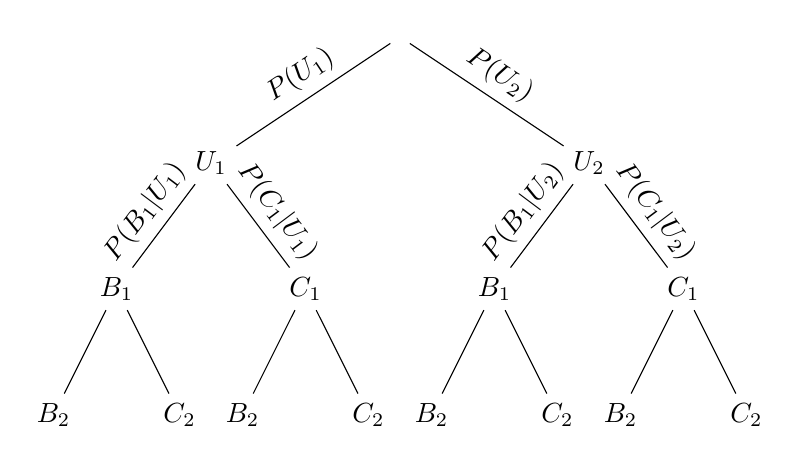
\begin{tikzpicture}[sloped,
                        level distance=2cm,
                        level 1/.style={sibling distance=6cm},
                        level 2/.style={sibling distance=3cm},
                        level 3/.style={sibling distance=2cm},
                        scale = 0.8]
    \node[] {}
    child {
        node[] {$U_1$}
        child {
          node[] {$B_1$}
          child {
            node[] {$B_2$}
          }
          child {
            node[] {$C_2$}
          }
          edge from parent
          node[above] {$P(B_1|U_1)$}
        }
        child {
          node[] {$C_1$}
          child {
            node[] {$B_2$}
          }
          child {
            node[] {$C_2$}
          }
          edge from parent
          node[above] {$P(C_1|U_1)$}
        }
        edge from parent
        node[above] {$P(U_1)$}
    }
    child {
        node[] {$U_2$}
        child {
          node[] {$B_1$}
          child {
            node[] {$B_2$}
          }
          child {
            node[] {$C_2$}
          }
          edge from parent
          node[above] {$P(B_1|U_2)$}
        }
        child {
          node[] {$C_1$}
          child {
            node[] {$B_2$}
          }
          child {
            node[] {$C_2$}
          }
          edge from parent
          node[above] {$P(C_1|U_2)$}
        }
        edge from parent
        node[above] {$P(U_2)$}
    };
    \end{tikzpicture}
    \end{center}
    Aby znaleźć $P(B_1\cap B_2)$ za pomocą powyższego drzewa, sumujemy $P(U_1\cap B_1\cap B_2)$ i $P(U_2\cap B_1\cap B_2)$, mnożąc liczby na odpowiednich ścieżkach w drzewie.
\end{example}

\subsection{Schemat Bernoulliego}

\textbf{Schematem Bernoulliego} nazywamy ciąg niezależnych powtórzeń tego samego doświadczenia, w którym możliwe są dwa wyniki: jeden z nich nazywamy \textbf{sukcesem} (o prawdopodobieństwie $p$), a drugi \textbf{porażką} (o prawdopodobieństwie $1 - p$). Pojedyncze doświadczenie nazywamy \textbf{próbą Bernoulliego}.

Taki schemat jest jednoznacznie określony przez podanie liczby prób (oznaczanej $n$) i prawdopodobieństwa sukcesu $p$. Można też rozpatrywać schematy Bernoulliego z nieskończoną liczbą prób.

Nietrudno kombinatorycznie pokazać, że prawdopodobieństwo uzyskania dokładnie $k$ sukcesów w schemacie Bernoulliego składającego się z $n$ prób wynosi
$$\purple{\binom{n}{k} p^k (1 - p)^{n - k}}$$
Istotnie, $k$ spośród $n$ prób zakończy się sukcesem (stanie się to z prawdopodobieństwem $p^k$), pozostałe $n - k$ prób zakończy się porażką (prawdopodobieństwo $(1 - p)^{n - k}$), a na $\binom{n}{k}$ sposobów wybieramy, które $k$ prób będzie pomyślne.

\begin{example}
    Rzucamy 10 razy kostką. Znajdziemy prawdopodobieństwo tego, że szóstka wypadnie raz lub dwa razy.

    Oznaczmy poszukiwane zdarzenie jako $A$. Mamy tu do czynienia ze schematem Bernoulliego składającym się z $n = 10$ prób. Próbą Bernoulliego jest pojedynczy rzut kostką, a sukcesem -- wyrzucenie 6 oczek, zatem $p = \frac{1}{6}$. Wobec tego obliczamy
    $$P(A) = \underbrace{\binom{10}{1} \left(\frac{1}{6}\right)^1 \left(\frac{5}{6}\right)^9}_{\text{jeden sukces}} + \underbrace{\binom{10}{2} \left(\frac{1}{6}\right)^2 \left(\frac{5}{6}\right)^8}_{\text{dwa sukcesy}}$$
\end{example}

\subsection{Niezależność zdarzeń}

Na ogół, jeśli zdarzenia $A, B$ są takie, że $P(B) > 0$, to prawdopodobieństwo warunkowe $P(A | B)$ różni się od prawdopodobieństwa bezwarunkowego $P(A)$. Innymi słowy, dodatkowa informacja podana za pomocą zdarzenia $B$ w istotny sposób zmienia szansę zajścia zdarzenia $A$. Czasami jednak to, czy zdarzenie $B$ zaszło czy nie, nie wpływa na prawdopodobieństwo $A$: mamy wtedy $P(A | B) = P(A)$. W takiej sytuacji mówimy, że $A$ i $B$ są \textbf{niezależne}.

Rozpisując wzór na prawdopodobieństwo warunkowe, powyższa równość daje się zapisać w równoważnej postaci stanowiącej definicję niezależności zdarzeń:
$$\purple{P(A \cap B) = P(A) \cdot P(B)}$$

Jeśli powyższa równość nie zachodzi, to powiemy, że zdarzenia $A$ i $B$ są \textbf{zależne}.

O pojęciu niezależności należy więc myśleć w sposób ,,czy zajście zdarzenia $B$ daje mi dodatkową informację na temat zdarzenia $A$?'', a nie w terminach związków fizycznych między zdarzeniami.

\begin{example}
    Z talii 52 kart losujemy kartę. Rozważmy zdarzenia:
    \begin{itemize}
        \item $A$ -- wylosowano króla,
        \item $B$ -- wylosowano kiera.
    \end{itemize}

    Wówczas zdarzenia $A$ i $B$ są niezależne -- łatwo sprawdzamy:
    $$P(A) = \frac{4}{52}, \qquad P(B) = \frac{13}{52} = \frac{1}{4}, \qquad P(A \cap B) = \frac{1}{52} = P(A)P(B)$$
\end{example}

\begin{exam}
    Rzucamy symetrycznymi kostkami: sześcienną i ośmiościenną. Niech $A$ będzie zdarzeniem, że na kostce sześciennej wypadło $6$. Zdarzeniami niezależnymi od $A$ są
    \answers{suma oczek na obu kostkach jest parzysta}{suma oczek na obu kostkach jest równa $7$}{suma oczek na obu kostkach jest większa od $7$}
    \bigskip

    Nietrudno zauważyć, że $|\Omega| = 48$ oraz $P(A) = \frac{1}{6}$. W każdym z podpunktów pozostaje nam zatem policzyć $P(A \cap B)$ oraz $P(B)$ (za $B$ oznaczamy zdarzenie z danego podpunktu), a następnie sprawdzić warunek na niezależność zdarzeń.
    \begin{enumerate}[\bf A.]
        \item Oznaczmy $B$ -- suma oczek na obu kostkach jest parzysta. Jeśli na pierwszej kostce wypadła parzysta liczba oczek, to na drugiej również, analogicznie dla nieparzystych. Mamy więc $|B| = 3 \cdot 4 + 3 \cdot 4 = 24$ oraz $P(B) = \frac{24}{48} = \frac{1}{2}$.
        
        Zdarzenie $A \cap B$ spełniają 4 zdarzenia elementarne: $(6, 2), (6, 4), (6, 6), (6, 8)$. W związku z tym
        $$P(A \cap B) = \frac{4}{48} = \frac{1}{12} = P(A) \cdot P(B)$$
        Zdarzenia $A$ i $B$ są więc niezależne. Intuicyjnie możemy rozumieć to następująco: nieważne, co wypadnie na pierwszej kostce, na drugiej jest zawsze tyle samo opcji.

        \item Oznaczmy $B$ -- suma oczek na obu kostkach jest równa 7. Nietrudno obliczamy:
        $$P(B) = \frac{6}{48}, \qquad P(A \cap B) = \frac{1}{48} = P(A) \cdot P(B)$$
        $A$ i $B$ ponownie są niezależne. Intuicyjnie: nieważne, co wypadnie na pierwszej kostce, na drugiej jest tylko jedna opcja.

        \item Oznaczmy $B$ -- suma oczek na obu kostkach jest większa od 7. Wypisując wszystkie zdarzenia elementarne spełniające ten warunek (pominiemy to w tym przykładzie), otrzymujemy
        $$P(B) = \frac{27}{48} = \frac{9}{16}, \qquad P(A \cap B) = \frac{7}{48} \neq P(A) \cdot P(B)$$
        Tym razem zdarzenia $A$ i $B$ są od siebie zależne. Intuicyjnie: zależnie od tego, co wypadnie na pierwszej kostce, na drugiej będziemy mieli różną liczbę opcji.
    \end{enumerate}
\end{exam}

Niezależność więcej niż dwóch zdarzeń definiujemy na dwa sposoby:
\begin{enumerate}
    \item Zdarzenia $A_1, A_2, ..., A_n$ są \textbf{niezależne parami}, jeśli każde dwa spośród nich są niezależne.

    \item Zdarzenia $A_1, A_2, ..., A_n$ są \textbf{niezależne} (lub \textit{niezależne łącznie}, bądź \textit{niezależne zespołowo}), jeśli dla dowolnego ciągu indeksów $i_1<i_2<\ldots<i_k$ zachodzi $$\purple{P(A_{i_1}\cap\ldots\cap A_{i_k})=P(A_{i_1})\cdot\ldots\cdot P(A_{i_k})}$$
\end{enumerate}

\begin{example}
    Rozważmy dwukrotny rzut sześcienną kostką i zbadajmy niezależność następujących trzech zdarzeń:
    \begin{itemize}
        \item $A$ -- suma oczek wynosi 7,
        \item $B$ -- w pierwszym rzucie uzyskano czwórkę,
        \item $C$ -- w drugim rzucie uzyskano trójkę.
    \end{itemize}

    Nietrudno sprawdzić, że $P(A) = P(B) = P(C) = \frac{1}{6}$. Zauważmy, że zdarzenia $A \cap B$, $A \cap C$, $B \cap C$ możemy zdefiniować tak samo: ,,w pierwszym rzucie wypadła czwórka, w drugim trójka'', stąd
    $$P(A \cap B) = P(A \cap C) = P(B \cap C) = \frac{1}{36}$$
    Widzimy więc, że zdarzenia $A, B, C$ są niezależne parami (każde dwa spośród nich są niezależne).
    \bigskip

    Z drugiej strony, $A \cap B \cap C$ również definiujemy jako ,,w pierwszym rzucie wypadła czwórka, w drugim trójka'', więc
    $$P(A \cap B \cap C) = \frac{1}{36} \neq P(A) \cdot P(B) \cdot P(C)$$
    Zdarzenia $A, B, C$ nie są więc niezależne.
\end{example}

\begin{problems}
    \prob Istnieje przestrzeń probabilistyczna $\Omega$ i zdarzenia $A,B\subseteq\Omega$ takie, że $P(A)=P(B)=\frac{2}{3}$ oraz
    \answers{$A$ i $B$ są niezależne}{$P(A|B)=\frac{1}{3}$}{$P(A|B)\neq P(B|A)$}

    \prob Chcemy rozpalić ognisko, lecz mamy do dyspozycji tylko trzy zapałki. Prawdopodobieństwo rozpalenia ogniska pojedynczą zapałką wynosi $0.4$, dwiema złączonymi zapałkami -- $0.6$, zaś trzema złączonymi zapałkami -- $0.8$. Żeby zmaksymalizować prawdopodobieństwo rozpalenia ogniska, należy
    \answers
    {użyć od razu trzech zapałek}
    {użyć najpierw dwóch zapałek, a potem jednej}
    {używać pojedynczych zapałek}

    \prob Rzucamy 10 razy symetryczną monetą. Wynika z tego, że
    \answers
    {prawdopodobieństwo, że wyrzucimy dokładnie 2 orły jest równe $\frac{45}{1024}$}
    {prawdopodobieństwo, że wyrzucimy orła w ostatnim rzucie pod warunkiem, że we wszystkich 10 rzutach wyrzucimy dokładnie 1 orła, jest równe $\frac{1}{2}$}
    {prawdopodobieństwo, że wyrzucimy orła w ostatnim rzucie pod warunkiem, że w pierwszych 9 rzutach wyrzucimy dokładnie 6 orłów, jest równe $\frac{1}{2}$}

    \prob Mamy 9 ponumerowanych kart od 1 do 9. Dwie osoby $A$ oraz $B$ losują bez zwracania po jednej karcie. Wygrywa osoba, która wylosuje kartę z większym numerem. Prawdą jest, że
    \answers{zdarzenia ,,wygrała osoba $A$'' oraz ,,osoba $A$ wylosowała kartę z numerem 5'' są niezależne}{zdarzenie ,,wygrała osoba $A$ pod warunkiem, że wylosowała kartę z numerem 7'' ma prawdopodobieństwo $\frac{3}{4}$}{zdarzenia ,,wygrała osoba $A$'' oraz ,,wygrała osoba $B$'' są niezależne}

    \prob Rzucamy symetryczną kostką dwudziestościenną. Niech $X$ będzie liczbą wyrzuconych oczek. Wtedy niezależne są zdarzenia ,,wyrzucono parzystą liczbę oczek'' oraz
    \answers
    {wyrzucono liczbę oczek podzielną przez $3$}
    {wyrzucono liczbę oczek podzielną przez $5$}
    {$X \leq 8$}
\end{problems}

\section{Dyskretne zmienne losowe}

W wielu sytuacjach, podczas przeprowadzania eksperymentu losowego, interesuje nas nie tyle konkretny wynik tego doświadczenia, co raczej jakaś charakterystyka liczbowa (ściślej: pewna funkcja od wyniku).

Przykładowo, rozważmy stukrotny rzut kostką i załóżmy, że interesuje nas zbadanie, czy suma wyrzuconych oczek wyniosła 200. Wówczas nie jest ważne, czy potencjalna dwusetka jest osiągana przez taki czy inny ciąg wyników -- liczy się tylko wspomniana suma. Wygodnie byłoby określić pewną funkcję $f : \Omega \to \RR$ zwracającą sumę wyrzuconych oczek i zbadać, z jakim prawdopodobieństwem wynik tej funkcji wynosi 200.

Każdą taką funkcję z $\Omega$ w $\RR$ nazywamy \textbf{zmienną losową}. Zazwyczaj zmienne losowe oznaczamy wielkimi literami $X, Y, Z, ...$

\begin{example}
    Rozważmy doświadczenie polegające na rzucie dwiema kostkami i sprawdźmy, w jaki sposób zmienne losowe mogą nam pomóc przy badaniu różnych jego własności.
    
    Przykładowo, zmienna losowa opisująca sumę oczek to funkcja $X((i,j)) = i + j$, podobnie można utworzyć funkcję dla iloczynu oczek, oczek na jednej z kostek itd.
    
    Zmiennej losowej można użyć do definiowania zdarzeń w jej dziedzinie, np.:
    \begin{itemize}
        \item $X = 5$ (suma oczek wynosi 5)
        \item $X \leq 4$ (suma oczek nie przekracza 4)
        \item $X \in \{3, 5, 7, 9, 11\}$ (suma oczek jest nieparzysta)
    \end{itemize}

    Możemy też definiować zdarzenia za pomocą kilku zmiennych, np. jeśli $Y$ to iloczyn oczek, to zdarzenie $X < Y$ oznacza sumę oczek mniejszą od iloczynu.
\end{example}

\subsection{Niezależność zmiennych losowych}

Zmienne losowe $X, Y$ są \textbf{niezależne}, gdy dla każdych $x,y\in\RR$ zachodzi
$$P(X=x \wedge Y=y) = P(X=x)P(Y=y)$$

\begin{example}
    Rozważmy dwukrotny rzut kostką oraz zmienne losowe:
    \begin{itemize}
        \item $X$ -- wynik pierwszego rzutu,
        \item $Y$ -- wynik drugiego rzutu,
        \item $Z$ -- suma liczb z obu rzutów.
    \end{itemize}

    Wówczas zmienne $X$ i $Y$ są niezależne: dla każdych $i, j \in \{1, ..., 6\}$ mamy
    $$P(X = i \land Y = j) = P(X = i) \cdot P(Y = j)$$

    Natomiast zmienne $X$ i $Z$ nie są niezależne, bo na przykład
    $$P(X = 1 \land Z = 12) = 0, \textqq{ale} P(X = 1) \cdot P(Z = 12) = \frac{1}{6} \cdot \frac{1}{36}$$

    Widzimy więc, że intuicja stojąca za niezależnością zmiennych losowych jest bardzo podobna jak ta, z którą mamy do czynienia przy niezależności zdarzeń.
\end{example}

\subsection{Rozkład zmiennej losowej}

Jeśli interesują nas własności zmiennej losowej $X$, to dziedzina oraz to, jak konkretnie $X$ jest zdefiniowana, nie mają dla nas znaczenia. Cała istotna informacja o zmiennej $X$ jest zawarta w jej \textbf{rozkładzie}.

\textbf{Rozkład zmiennej losowej} $X$ to zbiór par $(x_i, p_i)$, gdzie $x_i$ jest wartością zmiennej losowej $X$, a $p_i$ jest prawdopodobieństwem, że zmienna $X$ przyjmuje wartość $x_i$.

Jeśli $X$ i $Y$ mają ten sam rozkład, piszemy $\purple{X\sim Y}$.

\textbf{Rozkład dyskretny} zmiennej $X$ zachodzi, jeśli $\sum_{x\in\RR} P(X=x) = 1$, czyli z prawdopodobieństwem 1 zmienna $X$ przyjmuje jedną z przeliczalnie wielu wartości. Mówimy wtedy, że zmienna $X$ jest dyskretna.

\begin{example}
    Rozważmy trzykrotny rzut monetą i niech $X$ oznacza łączną liczbę orłów uzyskanych w tym doświadczeniu. Znajdziemy rozkład zmiennej $X$.

    Zmienna $X$ przyjmuje wartości w zbiorze $\{0, 1, 2, 3\}$, mamy:
    \begin{align*}
        &X((R, R, R)) = 0, \\
        &X((R, R, O)) = X((R, O, R)) = X((O, R, R)) = 1, \\
        &X((R, O, O)) = X((O, R, O)) = X((O, O, R)) = 2, \\
        &X((O, O, O)) = 3
    \end{align*}

    Łatwo wyznaczamy prawdopodobieństwa, z jakimi $X$ przyjmuje powyższe wartości:
    $$P(X = 0) = 1/8, \qquad P(X = 1) = 3/8, \qquad P(X = 2) = 3/8, \qquad P(X = 3) = 1/8.$$

    Równości te determinują rozkład zmiennej $X$. Łatwo możemy zwizualizować to na wykresie:
    \begin{center}
        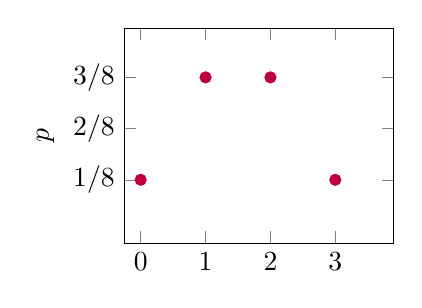
\begin{tikzpicture}
            \begin{axis}[
                width = 5cm,
                xmin = -0.25, xmax = 3.9,
                ymin = -0.03, ymax = 0.495,
                xtick distance = 1,
                ytick = {0.125, 0.25, 0.375},
                yticklabels = {$1/8$, $2/8$, $3/8$},
                ylabel = $p$
            ]
            \draw[purple, fill] (axis cs: 0, 0.125) circle (2pt);
            \draw[purple, fill] (axis cs: 1, 0.375) circle (2pt);
            \draw[purple, fill] (axis cs: 2, 0.375) circle (2pt);
            \draw[purple, fill] (axis cs: 3, 0.125) circle (2pt);
            \end{axis}
        \end{tikzpicture}
    \end{center}
\end{example}

\subsection{Podstawowe rozkłady dyskretne}

Opiszemy teraz pokrótce kilka podstawowych rozkładów zmiennych dyskretnych, pojawiających się stosunkowo często w rozmaitych przykładach i zastosowaniach.
\bigskip

Zmienna $X$ ma \textbf{rozkład dwumianowy} z parametrami $n,p$, oznaczany jako $\purple{X \sim \rpBinom(n,p)}$, jeśli 
$$P(X = k) = \binom{n}{k}p^k(1-p)^{n-k} \qquad \text{dla } k \in \{0,\ldots,n\}$$

Zmienna o rozkładzie dwumianowym opisuje \purple{liczbę sukcesów w schemacie $n$ prób Bernoulliego} o prawdopodobieństwie sukcesu $p$.

\begin{example}
    Rzucamy $n$ razy monetą, na której orzeł wypada z prawdopodobieństwem $p$. Jeśli zmienna $X$ oznacza liczbę orłów w takim ciągu rzutów, to ma ona rozkład dwumianowy:
    $$P(X = k) = \binom{n}{k} p^k (1-p)^{n-k} \qquad \text{dla } k \in \{0,\ldots,n\}$$

    Istotnie, jeśli w ciągu $n$ rzutów wypadło $k$ orłów, to takich różnych ciągów jest $\binom{n}{k}$ \gray{(wybieramy miejsca na orły, a w pozostałych $n - k$ miejscach wrzucamy reszki)}, przy czym każdy z nich mógł przytrafić się z prawdopodobieństwem $p^k (1 - p)^{n - k}$ \gray{($k$ razy wypadł orzeł i $n - k$ razy wypadła reszka)}.
\end{example}

Zmienna $X$ ma \textbf{rozkład geometryczny} z parametrem $p$, oznaczany jako $\purple{X \sim \rpGeom(p)}$, jeśli
$$P(X = k) = (1-p)^{k-1} \cdot p \qquad \text{dla } k \in \NN_+$$

Zmienna o rozkładzie geometrycznym opisuje \purple{numer pierwszej próby zakończonej sukcesem} w nieskończonym schemacie Bernoulliego o prawdopodobieństwie sukcesu $p$.

\begin{example}
    Rzucamy monetą, na której orzeł wypada z prawdopodobieństwem $p$, aż do uzyskania pierwszego orła. Jeśli zmienna $X$ oznacza liczbę rzutów w takim ciągu, to ma ona rozkład geometryczny: 
    $$P(X=k)=(1-p)^{k-1}\cdot p$$

    Istotnie, $X = k$ oznacza, że w $k - 1$ pierwszych rzutach musiała wypaść reszka (z prawdopodobieństwem $1 - p$), a w $k$-tym rzucie wypadł orzeł (z prawdopodobieństwem $p$).
\end{example}

Zmienna $X$ ma \textbf{rozkład Poissona} z parametrem $\lambda$, oznaczany jako $\purple{X \sim \rpPois(\lambda)}$, jeśli
$$P(X = k) = \frac{e^{-\lambda}\lambda^k}{k!} \qquad \text{dla } k \in \NN$$

Rozkład Poissona stosowany jest w rozmaitych kontekstach. Może być stosowany jako dobre przybliżenie rozkładu Bernoulliego $\rpBinom(n, p)$ w przypadku, gdy $n$ jest duże, $p$ jest małe, a $n \cdot p$ wynosi w przybliżeniu $\lambda$. Dzięki temu rozkład Poissona może być używany do badania zdarzeń ,,rzadkich'' i ,,całkowicie losowych'', na przykład:
\begin{itemize}
    \item przewidywanie liczby trzęsień ziemi na podstawie ich średnich wystąpień w przeszłości,
    \item szacowanie liczby błędów ortograficznych w książce o znanej liczbie znaków,
    \item zliczanie liczby telefonów odebranych w centrum obsługi klienta w ciągu godziny.
\end{itemize}

\begin{example}
    Kierownik laboratorium komputerowego otrzymuje średnio $\lambda$ informacji o awarii komputera na miesiąc. Znajdziemy rozkład zmiennej $X$ zliczającej liczbę otrzymanych takich informacji w miesiącu.

    Podzielmy miesiąc na $n$ przedziałów na tyle małych, że otrzymanie dwóch sygnałów w jednym przedziale jest zaniedbywalne (czyli $n\to\infty$). Ponadto, niech zdarzenia odpowiadające otrzymaniu awarii w dwóch różnych przedziałach będą niezależne. Mamy teraz do czynienia z ciągiem $n$ prób Bernoulliego, obliczymy więc prawdopodobieństwo sukcesu (otrzymania informacji o awarii w podanym przedziale).

    Skoro spośród $n$ przedziałów średnio $\lambda$ z niech zawiera awarię, to prawdopodobieństwo wynosi $p = \frac{\lambda}{n}$ i wtedy $X \sim \rpBinom(n,\frac{\lambda}{n})$ dla dużych $n$, czyli
    $$P(X = k) = \binom{n}{k}\left(\frac{\lambda}{n}\right)^k\left(1-\frac{\lambda}{n}\right)^{n-k}$$
    Dla $n \to \infty$ wyrażenie to zbiega do $e^{-\lambda}\lambda^k/k!$, więc (wprost z definicji) $X$ ma rozkład Poissona z parametrem $\lambda$.
\end{example}

\section{Parametry rozkładu}

W tym rozdziale przyjrzymy się kilku istotnym parametrom rozkładów zmiennych losowych, pozwalającym nam na analizowanie ich rozmaitych własności.

\subsection{Wartość oczekiwana}

Niech $X$ będzie zmienną losową o rozkładzie dyskretnym. \textbf{Wartością oczekiwaną} (średnią) $X$ nazywamy wartość sumy
$$
\purple{\E X = \sum_{x\in\RR} \big(x \cdot P(X = x)\big)}
$$

Wartość oczekiwana ma bardzo naturalną fizyczną interpretację: jest to ważona średnia wartości, które mogą być przyjęte przez daną zmienną, gdzie każda wartość ma wagę odpowiadającą jej prawdopodobieństwu.

\begin{example}
    Dysponujemy fałszywą kostką, w której na ścianie z trzema oczkami domalowano dwa dodatkowe oczka. Wyznaczymy wartość oczekiwaną liczby wyrzuconych oczek na tej kostce.

    Oznaczmy odpowiednią zmienną jako $X$. Nietrudno znaleźć jej rozkład:
    $$P(X = k) = \begin{cases}
        1/3 & \text{dla } k = 5 \\
        1/6 & \text{dla } k = 1, 2, 4, 6
    \end{cases}$$

    Szukana przez nas wartość oczekiwana $X$ wynosi więc
    $$\E X = 1 \cdot P(X = 1) + 2 \cdot P(X = 2) + 4 \cdot P(X = 4) + 5 \cdot P(X = 5) + 6 \cdot P(X = 6) =$$ $$= \frac{1}{6}(1 + 2 + 4 + 6) + \frac{1}{3} \cdot 5 = \frac{23}{6}$$
\end{example}

Niekiedy zdarza się, że dysponujemy pewną zmienną losową i interesuje nas nie tyle średnia tej zmiennej, co średnia \textit{pewnej funkcji} tej zmiennej; innymi słowy, mamy zadaną pewną funkcję $f : \RR \to \RR$ i naszym celem jest wyznaczenie $\E f(X)$. Wówczas możemy skorzystać z następującego faktu:
$$\E f(X) = \sum_{x \in \RR} \big(f(x) \cdot P(X = x)\big)$$

\begin{example}
    Losujemy liczbę ze zbioru $\{1, 2, ..., 10\}$. Obliczymy średnią odległość tej liczby od 2.

    Jeśli przez $X$ oznaczymy wylosowaną liczbę, to naszym celem jest obliczenie $\E |X - 2|$. Ponieważ rozkład $X$ to
    $$P(X = j) = 1/10 \qquad \text{dla } j = 1, 2, ..., 10,$$
    na mocy powyższego twierdzenia zachodzi
    $$\E |X - 2| = \sum_{j = 1}^{10} |j - 2| \cdot P(X = j) = \frac{1}{10} \sum_{j = 1}^{10} |j - 2| = \frac{1}{10} + \frac{1}{10} \sum_{j = 3}^{10} |j - 2| = \frac{1}{10} + \frac{36}{10} = 3.7$$
\end{example}

Wartość oczekiwana ma własność \purple{liniowości}, tj. dla dowolnych zmiennych $X, Y$ oraz dowolnego $c \in \RR$ mamy:
\begin{itemize}
    \item $\E (cX) = c \cdot \E X$
    \item $\E (X+Y) = \E X + \E Y$
\end{itemize}

Jeśli $X,Y$ są niezależnymi zmiennymi losowymi (dyskretnymi), to dodatkowo zachodzi \purple{multiplikatywność}: $$\E (XY) = \E X \cdot \E Y$$

\begin{example}
    Rzucono $n$ razy kostką do gry. Obliczymy wartość oczekiwaną łącznej liczby wyrzuconych oczek.

    Oznaczmy szukaną sumę jako $X$. Można próbować obliczyć średnią $X$ bezpośrednio z definicji, ale to bardzo żmudne podejście, gdyż wyznaczenie rozkładu $X$ jest niełatwym zagadnieniem kombinatorycznym.
    
    Aby uniknąć tego problemu, rozbijemy $X$ na sumę prostszych zmiennych: dla $i = 1, 2, ..., n$ przez $X_i$ oznaczymy liczbę oczek wyrzuconych w $i$-tym rzucie. Wówczas $X = X_1 + X_2 + ... + X_n$ oraz 
    $$\E X_i = 1 \cdot P(X_i = 1) + 2 \cdot P(X_i = 2) + ... + 6 \cdot P(X_i = 6) = \frac{7}{2}$$
    i możemy skorzystać z liniowości wartości oczekiwanej:
    $$\E X = \E X_1 + \E X_2 + ... + \E X_n = \frac{7n}{2}$$
\end{example}

\subsection{Wariancja i odchylenie standardowe}

Niech $X$ będzie zmienną losową o skończonej wartości oczekiwanej. \textbf{Wariancję} $X$ definiujemy wzorem
$$\Var X = \E (X - \E X)^2$$

\textbf{Odchyleniem standardowym} zmiennej $X$ nazywamy liczbę $\sigma(X) = \sqrt{\Var X}$.

Przeprowadzając proste przekształcenia, łatwo wyprowadzić alternatywny wzór na wariancję
$$\Var X = \E (X^2) - (\E X)^2,$$
który w wielu sytuacjach oferuje najprostszy sposób jej obliczenia.
\bigskip

O ile wartość oczekiwana mówi nam o tym, jaka jest średnia wartość zmiennej $X$, tak wariancja odpowiada za ,,rozrzut'' jej różnych wartości. Aby lepiej zrozumieć intuicję za tym stojącą, rozważmy trzy zmienne losowe:
\begin{align*}
    X &= 0, \\
    Y & = \begin{cases}
        1 & \text{z prawdopodobieństwem } 1/2, \\
        -1 & \text{z prawdopodobieństwem } 1/2, \\
    \end{cases} \\
    Z & = \begin{cases}
        100 & \text{z prawdopodobieństwem } 1/2, \\
        -100 & \text{z prawdopodobieństwem } 1/2.
    \end{cases}
\end{align*}

Z punktu widzenia wartości oczekiwanej, te zmienne nie różnią się między sobą -- wszystkie mają średnią równą 0. Tym niemniej jest intuicyjnie jasne, że pierwsza z nich nie ma żadnego rozrzutu, druga z nich ma ,,umiarkowany'' rozrzut, a trzecia z nich wykazuje największe odchylenia od swojej wartości oczekiwanej.

Można by się też zastanowić, dlaczego nie definiujemy wariancji bardziej oczywistym (intuicyjnie) wzorem $\E |X - \E X|$, mierzącym wprost jej średnie odchylenie od wartości oczekiwanej? Okazuje się, że tak zdefiniowana wariancja nie jest wygodna -- nie posiada pewnych specjalnych algebraicznych własności. Stąd znacznie lepszym pomysłem jest mierzenie odchylenia w sensie średniokwadratowym $\E (X - \E X)^2$.

\begin{example}
    Ze zbioru $\{1, 2, ..., n\}$ losujemy liczbę $X$. Obliczymy wariancję $X$.

    Rozkład zmiennej $X$ zadany jest przez równości
    $$P(X = k) = 1/n \qquad \text{dla } k = 1, 2, ..., n,$$
    więc
    $$\E X = \sum_{k = 1}^{n} \big(k \cdot P(X = k)\big) = \frac{1}{n} \sum_{k = 1}^{n} k = \frac{n + 1}{2}$$
    i analogicznie
    $$\E (X^2) = \sum_{k = 1}^{n} \big(k^2 \cdot P(X = k)\big) = \frac{1}{n} \sum_{k = 1}^{n} k^2 = \frac{(n + 1)(2n + 1)}{6}$$
    Wobec tego
    $$\Var X = \E (X^2) - (\E X)^2 = \frac{(n + 1)(2n + 1)}{6} - \left(\frac{n + 1}{2}\right)^2 = \frac{n^2 - 1}{12}$$

    Wynika stąd, że dla danego $n$ zmienna $X$ średnio ,,odchyla się'' od swojej wartości oczekiwanej o $\sqrt{\frac{n^2 - 1}{12}}$.
\end{example}

Jeśli zmienne losowe $X$ i $Y$ są niezależne i mają skończoną wariancję, to jest ona \purple{addytywna}:
$$
\Var (X+Y) = \Var X + \Var Y
$$

Ponadto, bezpośrednio z definicji, wariancja posiada następującą własność: jeśli $X$ jest zmienną losową o skończonej wartości oczekiwanej oraz $a, b$ są liczbami rzeczywistymi, to
$$\Var (aX + b) = a^2 \Var X$$

\begin{example}
    Rzucamy trzy razy monetą i przez $X$ oznaczamy różnicę między liczbą wyrzuconych reszek i orłów. Obliczymy wartość oczekiwaną i wariancję $X$.

    Niech $R$ będzie liczbą wyrzuconych reszek, a $O$ -- liczbą orłów. Jasne jest, że $R + O = 3$ oraz $X = R - O$, skąd bezpośrednio wynika, że $X = 2R - 3$. Łatwo wyznaczymy też rozkład $R$:
    $$P(R = 0) = \frac{1}{8}, \qquad P(R = 1) = \frac{3}{8}, \qquad P(R = 2) = \frac{3}{8}, \qquad P(R = 3) = \frac{1}{8}$$

    Wobec tego, korzystając z liniowości wartości oczekiwanej:
    $$\E X = \E (2R - 3) = 2 \E R - \E 3 = 2 \left(0 \cdot \frac{1}{8} + 1 \cdot \frac{3}{8} + 2 \cdot \frac{3}{8} + 3 \cdot \frac{1}{8}\right) - 3 = 0$$
    \gray{(dygresja: wynik ten jest intuicyjnie oczywisty, średnio liczba reszek i orłów jest ta sama i wynosi 1.5)}

    Ponadto, korzystając z podanej wcześniej własności wariancji,
    $$\Var X = \Var (2R - 3) = 4 \Var R$$

    Jak już obliczyliśmy wcześniej, $\E R = 1.5$ oraz
    $$\E R^2 = 0^2 \cdot \frac{1}{8} + 1^2 \cdot \frac{3}{8} + 2^2 \cdot \frac{3}{8} + 3^2 \cdot \frac{1}{8} = 3$$

    Ostatecznie mamy więc
    $$\Var X = 4 \Var R = 4 (\E (R^2) - (\E R)^2) = 3$$
\end{example}

\subsection{Wartości parametrów znanych rozkładów dyskretnych}

Poniższa tabela przedstawia spis wartości oczekiwanych i wariancji dla znanych nam rozkładów dyskretnych. Wszystkie z nich można w łatwy sposób wyprowadzić wprost z definicji, większość powinna również intuicyjnie wynikać z interpretacji kombinatorycznych poszczególnych rozkładów.

\begin{center}
\renewcommand{\arraystretch}{1.5}
\newcolumntype{C}{>{\centering\arraybackslash} m{3cm}}
\begin{tabular}{ C | C | C }
    & $\E X$ & $\Var X$ \\ \hline
    $X \sim \rpBinom(n, p)$ & $np$ & $np(1 - p)$ \\ \hline
    $X \sim \rpGeom(p)$ & $1/p$ & $(1 - p)/p^2$ \\ \hline
    $X \sim \rpPois(\lambda)$ & $\lambda$ & $\lambda$
\end{tabular}
\end{center}

\subsection{Funkcje tworzące prawdopodobieństwa}

Niech $X$ będzie zmienną losową o wartościach naturalnych. \textbf{Funkcją tworzącą prawdopodobieństwa} zmiennej $X$ jest
$$
g_X(t) = \sum_{k=0}^\infty P(X=k)\cdot t^k
$$

Za pomocą funkcji tworzących możemy łatwo obliczać wartość oczekiwaną i wariancję:
$$
\E X = g_X'(1), \qquad \Var X = g_X''(1) + g_X'(1) - g_X'^2(1),
$$
o ile te wartości istnieją i są skończone. Wzory te wynikają wprost z definicji wartości oczekiwanej i wariancji.

\begin{example}
    Znajdziemy funkcję tworzącą prawdopodobieństwa zmiennej $X$ o rozkładzie dwumianowym $\rpBinom(n, p)$.

    Mamy $P(X = k) = \binom{n}{k} p^k (1 - p)^{n - k}$, więc
    $$g_X(t) = \sum_{k = 0}^{n} \binom{n}{k} p^k (1 - p)^{n - k} t^k = \big(pt + (1 - p)\big)^n = (pt - p + 1)^n$$

    Dzięki takiej funkcji łatwo wyprowadzimy wzory na $\E X$ oraz $\Var X$. Zaczniemy od wyznaczenia wzoru na pierwszą i drugą pochodną:
    $$g'_X(t) = np(pt - p + 1)^{n - 1}, \qquad g''_X(t) = n(n - 1)p^2(pt - p + 1)^{n - 2},$$
    skąd otrzymujemy
    $$\E X = g'_X(1) = np, \qquad \Var X = \purple{g_X''(1)} + \teal{g_X'(1)} - \orange{g_X'^2(1)} = \purple{n(n - 1)p^2} + \teal{np} - \orange{n^2p^2} = np - np^2 = np(1 - p)$$
\end{example}

Jeśli $X$ jest zmienną losową o wartościach naturalnych oraz $c$ jest liczbą naturalną, to łatwo możemy wyznaczyć funkcję zmiennej $cX$:
$$g_{cX}(t) = g_X(t^c)$$

Jeśli natomiast $X$ i $Y$ są \purple{niezależnymi} zmiennymi o wartościach naturalnych, to funkcja tworząca prawdopodobieństwa sumy tych zmiennych jest równa
$$g_{X + Y}(t) = g_X(t) \cdot g_Y(t)$$

\begin{example}
    Ponownie obliczymy funkcję tworzącą prawdopodobieństwa dla zmiennej $X$ o rozkładzie dwumianowym $\rpBinom(n, p)$, tym razem rozbijając ją na niezależne zmienne $X_i$ reprezentujące poszczególne próby Bernoulliego w całym schemacie.

    Mamy więc $X = X_1 + X_2 + ... + X_n$, gdzie $P(X_i = 1) = p$ oraz $P(X_i = 0) = 1 - p$. Funkcją tworzącą prawdopodobieństwa dla zmiennych $X_i$ jest
    $$g_{X_i}(t) = P(X_i = 0) t^0 + P(X_i = 1) t^1 = (1 - p) + pt = pt - p + 1,$$
    a skoro $X$ to suma $n$ niezależnych zmiennych o takim rozkładzie, to
    $$g_X(t) = \big(g_{X_i}(t)\big)^n = (pt - p + 1)^n$$
\end{example}

\begin{problems}
    \prob Wrzucamy losowo dwie kule do dwóch urn. Wartość oczekiwana liczby niepustych urn jest równa
    \answers
    {1}
    {$\frac{3}{2}$}
    {$2(1 - \frac{1}{e})$}

    \prob Wrzucamy do worka $n \geq 3$ kul, każdą z nich malujemy niezależnie z prawdopodobieństwem $\frac{1}{2}$ na biało. Wartość oczekiwana liczby białych kul
    \answers{wynosi $\frac{n(n-1)}{2}$}{wynosi $\frac{n}{2}$}{jest większa lub równa wariancji liczby białych kul}

    \prob Dany jest generator bitów, dla którego każdy kolejny wygenerowany bit jest jedynką z prawdopodobieństwem 0.5. Niech $X$ będzie zmienną losową oznaczająca liczbę wygenerowanych jedynek przez ten generator w 100 próbach. Nie wiadomo, czy kolejne losowania są niezależne. Wówczas
    \answers{$\mathrm{E}X = 50$}{$\mathrm{E}X = 50$, gdy kolejne bity są generowane niezależnie}{$\mathrm{Var}(X) = 25$}

    \prob Niech $X$ i $Y$ to zmienne losowe, takie że $\E X = 1$, $\Var X = 4$ i $Y = 2X + 3$. Wtedy
    \answers{$\E Y = 4$}{$\sigma(Y) = 4$}{$\Var Y = 4$}

    \prob Niech $X$ i $Y$ będą zdarzeniami niezależnymi, wtedy
    \answers
    {$\mathrm{E}(X - Y) = \mathrm{E}X - \mathrm{E}Y$}
    {$\mathrm{E}(XY) = \mathrm{E}X \cdot \mathrm{E}Y$}
    {$\mathrm{E}(X / Y) = \mathrm{E}X / \mathrm{E}Y$}

    \prob Niech $X$ i $Y$ będą zmiennymi losowymi o wartościach nieujemnych. Wynika z tego, że
    \answers{$\mathrm{E}(XY)=\mathrm{E}X\cdot \mathrm{E}Y$, jeśli $X$ i $Y$ są niezależne}{$\mathrm{E}(\min(X,Y))=\min(\mathrm{E}X,\mathrm{E}Y)$}{$\mathrm{E}(\min(X,Y))=\min(\mathrm{E}X,\mathrm{E}Y)$, jeśli $X$ i $Y$ są niezależne}
\end{problems}

\section{Nierówności probabilistyczne}

W rachunku prawdopodobieństwa czy statystyce często nie jest możliwe dokładne wyliczenie pewnych interesujących nas wartości. Niemniej jednak, w wielu zastosowaniach istotna jest nie tyle dokładna wartość, co jej oszacowanie.

Przykładowo, gracza może interesować, czy prawdopodobieństwo, że przegra, jest mniejsze niż pewna z góry ustalona liczba i na tej podstawie może podjąć decyzję, czy wziąć udział w grze. Podobnie przy badaniach statystycznych ważne jest oszacowanie prawdopodobieństwa, że błąd wyniesie mniej niż interesująca nas dokładność.

Ogólniej: jeśli przez $X$ oznaczymy losowy błąd danej metody pomiarowej, jesteśmy zainteresowani nierównościami postaci $P(X \geq x) \leq c$, gdzie $c$ jest pewnym ustalonym parametrem.
\bigskip

Podstawowym narzędziem matematycznym służącym do uzyskiwania nierówności powyższego typu jest \textbf{nierówność Markowa}: dla dowolnej nieujemnej zmiennej losowej $X$ oraz dla każdego $c > 0$ zachodzi
$$\purple{P(X \geq c) \leq \frac{\E X}{c}}$$

\begin{example}
    Oszacujemy prawdopodobieństwo uzyskania w 1000 rzutach monetą przynajmniej 750 orłów.
    
    Niech $X_1, X_2, ... ,X_{1000}$ będą wynikami kolejnych rzutów (1 dla orła, 0 dla reszki). Wtedy $X = \sum_{i=1}^{1000} X_i$ jest liczbą wszystkich orłów. Jasne jest też, że $X \sim \rpBinom(1000, \frac{1}{2})$.

    Ponieważ dla rozkładu dwumianowego $\E X = 1000 \cdot \frac{1}{2} = 500$, to z nierówności Markowa otrzymujemy
    $$
    P(X \geq 750) = P\left(X \geq \frac{3}{2} \E X\right) \leq \frac{2}{3}
    $$
    
    Widzimy, że to niezbyt imponujące oszacowanie (intuicyjnie wynik powinien być dużo niższy).
\end{example}

Nierówność Markowa, choć niezwykle prosta, ma bardzo dużo zastosowań. Jej siła wynika między innymi z faktu, że możemy zastosować ją nie tylko do zmiennej losowej $X$, którą jesteśmy zainteresowani, ale także do zmiennych postaci $f(X)$, uzyskując nowe nierówności.

Na przykład, podstawiając zmienną $(X - \E X)^2$ do nierówności Markowa, uzyskamy \textbf{nierówność Czebyszewa}: dla dowolnej nieujemnej losowej $X$ oraz dla każdego $c > 0$ zachodzi
$$
\purple{P(|X - \E X| \geq c) \leq \frac{\Var X}{c^2}}
$$

\begin{example}
    Kontynuujemy poprzedni przykład. Tym razem oszacujemy prawdopodobieństwo uzyskania co najmniej 750 orłów w ciągu 1000 rzutów monetą za pomocą nierówności Czebyszewa.

    Dla zmiennej $X$ o rozkładzie dwumianowym mamy $\E X = 1000 \cdot \frac{1}{2} = 500$ oraz $\Var X = 1000 \cdot \frac{1}{2} \cdot (1 - \frac{1}{2}) = 250$.
    
    Nierówność Czebyszewa pozwoli nam na oszacowanie prawdopodobieństwa $P(|X - 500| \geq c)$ dla pewnej ustalonej liczby $c \in \RR$. Aby móc otrzymać z tego $P(X \geq 750)$, skorzystamy z faktu, że w schemacie Bernoulliego (u nas: 1000 rzutów monetą) zachodzi symetria $P(X \geq 750) = P(X \leq 250)$, co pozwala nam uzyskać równość
    $$P(|X - 500| \geq 250) = P(X \geq 750) + P(X \leq 250) = 2 \cdot P(X \geq 750),$$
    więc mamy
    $$
    P(X \geq 750) = \frac{1}{2} \cdot P(|X - 500| \geq 250) \leq \frac{1}{2} \cdot \frac{250}{250^2} = \frac{1}{500}
    $$
    
    Widzimy, że to dużo lepsze oszacowanie niż poprzednio.
\end{example}

% TODO
\begin{editorsnote}
    W rozdziale brakuje informacji na temat nierówności Chernoffa (jest ona wspomniana w podstawie programowej), jednak zawarta tu teoria jest wystarczająca do rozwiązania zadań z przeanalizowanych na potrzeby tego repetytorium archiwalnych egzaminów.
\end{editorsnote}

\begin{problems}
    \prob Niech $X$ będzie zmienną losową reprezentującą długość trwania programu dla różnych wejść, niech $\mu$ to wartość oczekiwana $X$, zaś $\sigma$ to odchylenie standardowe. Prawdą jest, że
    \answers{$P(X > 2\mu) \leq \frac{1}{4}$}{$P(X > \mu + 2\sigma) \leq \frac{1}{4}$}{$P(X > 100\mu) \leq \frac{1}{10^{10}}$}
\end{problems}

\section{Ciągły rozkład prawdopodobieństwa}

Dla dyskretnych zmiennych losowych mieliśmy $\sum_{x \in \RR} P(X = x) = 1$, czyli suma prawdopodobieństw przeliczalnie wielu wartości uzyskiwanych przez zmienną jest równa 1. Zauważmy jednak, że taka zmienna nie pozwoliłaby nam rozpatrzeć doświadczenia polegającego na wylosowaniu punktu z odcinka $[0, 1]$ -- ponieważ zbiór ten jest nieprzeliczalny, a każdy punkt równo prawdopodobny do wylosowania, nie potrafilibyśmy określić prawdopodobieństwa wylosowania pojedynczego punktu, tak żeby wszystkie z nich zsumowały się do 1.

Podobnie jest w każdej sytuacji, w której wynikiem jakiegoś doświadczenia może być dowolna liczba rzeczywista, np. pomiar wzrostu osoby lub prędkości samochodu. Mamy tu do czynienia z \textbf{ciągłym rozkładem prawdopodobieństwa} i w tym rozdziale zobaczymy, jak sobie z nim poradzić.

\subsection{Prawdopodobieństwo geometryczne}

O ile w problemach dyskretnych korzystamy zazwyczaj ze schematu klasycznego, tak w doświadczeniach losowych o charakterze ciągłym przydatne może okazać się \textbf{prawdopodobieństwo geometryczne}. Najprostszym przykładem jest losowanie punktu z pewnego zbioru $\Omega$.

Załóżmy, że $\Omega$ jest pewnym podzbiorem przestrzeni $\RR^d$ i ma skończoną miarę (długość, pole powierzchni, objętość... -- w zależności od wymiaru $d$). Wówczas prawdopodobieństwo dowolnego zdarzenia $A \subseteq \Omega$ jest \purple{proporcjonalne do jego miary}:
$$P(A) = \frac{|A|}{|\Omega|}$$

\begin{example}
    Z przedziału $[0, 1]$ wybieramy losowo dwie liczby. Jakie jest prawdopodobieństwo tego, że obie te liczby są mniejsze niż $1/2$?

    Zastosujemy prawdopodobieństwo geometryczne. Oznaczmy wybrane liczby przez $x, y$. Wówczas
    $$\Omega = \{(x, y) \ | \ x, y \in [0, 1]\} = [0, 1]^2$$

    Następnym krokiem jest zinterpretowanie badanego zdarzenia $A$ jako podzbioru $\Omega$. Mamy
    $$A = \left\{(x, y) \in \Omega \ | \ x, y \leq \frac{1}{2}\right\} = \left[0, \frac{1}{2}\right]^2,$$
    a zatem obliczając pola powierzchni odpowiednich zbiorów:
    $$P(A) = \frac{|A|}{|\Omega|} = \frac{1}{4}$$

    Możemy to łatwo zwizualizować w układzie współrzędnych:
    \begin{center}
        \begin{tikzpicture}
            \begin{axis}[
                width = 5 cm,
                xmin = -0.25, xmax = 1.25,
                ymin = -0.25, ymax = 1.25,
                xtick distance = 0.5,
                ytick distance = 0.5,
            ]
                \addplot [
                    draw=purple,
                    fill=purple,
                    fill opacity=0.3,
                ] coordinates {(0, 0) (1, 0) (1, 1) (0, 1) (0, 0)};
                
                \addplot [
                    draw=teal,
                    pattern=north west lines,
                    pattern color=teal,
                ] coordinates {(0, 0) (0.5, 0) (0.5, 0.5) (0, 0.5) (0, 0)};
                
                \node at (axis cs: 0.75, 0.75) {\textcolor{purple}{$\Omega$}};
                \node at (axis cs: 0.25, 0.25) {$A$};
            \end{axis}
        \end{tikzpicture}
    \end{center}
\end{example}

\subsection{Ciągłe zmienne losowe}

Zmienna $X$ ma \textbf{rozkład ciągły}, jeśli istnieje funkcja $f_X : \RR \to \RR_{\geq0}$, taka że dla każdego przedziału $[a, b]$ zachodzi
$$P(X \in [a, b]) = \int_a^b f_X(x) \dx$$

Funkcja $f_X$ w powyższej definicji to \textbf{funkcja gęstości} zmiennej $X$. Dla zmiennej ciągłej prawdopodobieństwo, że zmienna przyjmie wartość między $a$ i $b$ jest równe polu powierzchni pod krzywą gęstości nad tym odcinkiem:

\begin{center}
    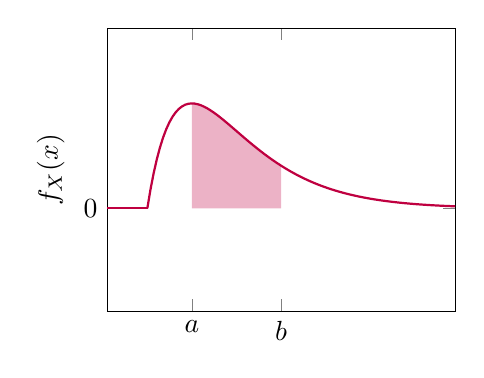
\begin{tikzpicture}
        \begin{axis}[
            width = 6cm,
            xmin = -0.9, xmax = 6.9,
            ymin = -0.4, ymax = 0.7,
            xtick = {1, 3},
            xticklabels = {$a$, $b$},
            ylabel = $f_X(x)$,
            ytick distance = 1,
            samples = 100
        ]
            \addplot[thick, purple, domain = -1:0] {0};
            \addplot[draw = none, fill = purple!30, domain = 1:3] {0.15 * x * e^(-(x-2))} \closedcycle;
            \addplot[thick, purple, domain = 0:7] {0.15 * x * e^(-(x-2))};
        \end{axis}
    \end{tikzpicture}
\end{center}

Oczywiste jest również, że prawdopodobieństwa wszystkich możliwych wartości $X$ muszą sumować się do 1, w związku z czym dla każdej funkcji gęstości mamy
$$\int_{-\infty}^{+\infty} f_X(x) \dx = 1$$

\begin{example}
    Rzucamy niesymetryczną monetą, na której prawdopodobieństwo wypadnięcia orła wynosi 1/3. Jeśli wypadnie orzeł, to losujemy punkt $X$ z odcinka $[-2, 0)$, a jeśli wypadnie reszka, to losujemy $X$ z odcinka $[0, 3]$. Wyznaczymy funkcję gęstości zmiennej $X$.

    Żeby $X$ przyjęło jedną z wartości z przedziału $[-2, 0)$, na monecie musi wypaść orzeł (z prawdopodobieństwem 1/3). Ponieważ wylosowanie każdego punktu jest równie prawdopodobne, dla $x \in [-2, 0)$ mamy
    $$f_X(x) = \frac{1}{3} \cdot \frac{1}{0 - (-2)} = \frac{1}{6}$$

    Analogicznym rozumowaniem dla reszki i przedziału $[0, 3]$ dochodzimy do wniosku, że funkcją gęstości zmiennej $X$ jest
    $$
    f_X(x) = \begin{cases}
        \frac{1}{6} & \text{dla } x \in [-2, 0), \\
        \frac{2}{9} & \text{dla } x \in [0, 3], \\
        0 & \text{wpp.}
    \end{cases}
    $$

    Oznacza to, że $X$ przyjmie wartość z przedziału $[-2, 0)$ z prawdopodobieństwem 1/6 oraz wartość z przedziału $[0, 3]$ z prawdopodobieństwem 2/9. Możemy zobrazować $f_X$ w układzie współrzędnych:
    \begin{center}
        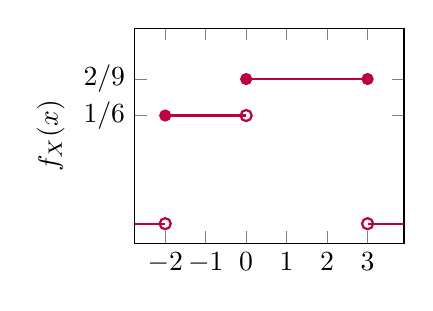
\begin{tikzpicture}
            \begin{axis}[
                width = 5cm,
                xmin = -2.75, xmax = 3.9,
                ymin = -0.03, ymax = 0.3,
                xtick distance = 1,
                ylabel = $f_X(x)$,
                ytick = {0.166, 0.222},
                yticklabels = {$1/6$, $2/9$}
            ]
            \addplot[thick, purple, domain = -3:-2] {0};
            \addplot[thick, purple, domain = -2:0] {0.166};
            \addplot[thick, purple, domain = 0:3] {0.222};
            \addplot[thick, purple, domain = 3:4] {0};
            \draw[purple, thick] (axis cs: -2, 0) circle (2pt);
            \draw[purple, fill] (axis cs: -2, 0.166) circle (2pt);
            \draw[purple, thick] (axis cs: 0, 0.166) circle (2pt);
            \draw[purple, fill] (axis cs: 0, 0.222) circle (2pt);
            \draw[purple, fill] (axis cs: 3, 0.222) circle (2pt);
            \draw[purple, thick] (axis cs: 3, 0) circle (2pt);
            \end{axis}
        \end{tikzpicture}
    \end{center}

    Z rysunku nietrudno przekonać się też, że
    $$\int_{-\infty}^{\infty} f_X(x) = 2 \cdot \frac{1}{6} + 3 \cdot \frac{2}{9} = 1,$$
    co potwierdza dobre zdefiniowanie funkcji gęstości.
\end{example}

Znany jest jeszcze jeden ważny fakt dotyczący rozkładu sum niezależnych zmiennych losowych o rozkładzie ciągłym.

Załóżmy, że $X, Y$ są \purple{niezależnymi} ciągłymi zmiennymi losowymi z gęstościami $f_X, f_Y$. Wówczas zmienna $X + Y$ ma rozkład z gęstością będącą splotem funkcji $f_X$ i $f_Y$:
$$f_{X + Y}(x) = \int_{-\infty}^{+\infty} f_X(y) f_Y(x - y) \dy$$

\subsection{Dystrybuanta}

W przypadku doświadczeń losowych o charakterze ciągłym z reguły jesteśmy zainteresowani zdarzeniami typu $P(X \leq c)$ dla pewnej zmiennej losowej $X$ i liczby rzeczywistej $c$.

\textbf{Dystrybuanta} zmiennej losowej $X$ to funkcja $F_X : \RR \to [0, 1]$ określona jako $$F_X(x) = P(X \leq x)$$

Nietrudno zauważyć, że dystrybuanta jest ściśle powiązana z funkcją gęstości, przez co \purple{jednoznacznie determinuje rozkład} dowolnej zmiennej losowej.

Co ważne: dystrybuanta nie jest związana wyłącznie z pojęciem rozkładu ciągłego i może być stosowana także do innych zmiennych.

\begin{example}
    Rozważmy (dyskretną) zmienną losową dwupunktową, przyjmującą wartości $1$ i $-1$, każdą z prawdopodobieństwem 1/2. Jej dystrybuantą jest funkcja
    $$F(x) = \begin{cases}
        0 & \text{dla } x \in (-\infty, -1), \\
        \frac{1}{2} & \text{dla } x \in [-1, 1), \\
        1 & \text{dla } x \in [1, \infty).
    \end{cases}$$
\end{example}

Możemy zauważyć, że nie każda funkcja może być dystrybuantą -- ma to związek ze znanymi nam podstawowymi własnościami prawdopodobieństwa. W szczególności wyróżniamy następujące \purple{własności dystrybuanty}:
\begin{enumerate}
    \item $F_X$ jest niemalejąca,
    \item $F_X$ jest prawostronnie ciągła,
    \item $\Lim_{x \to -\infty} F_X(x) = 0$ oraz $\Lim_{x \to +\infty} F_X(x) = 1$.
\end{enumerate}

Dodatkowo, \purple{jeśli $X$ jest zmienną ciągłą, to $F_X$ jest funkcją ciągłą}.
\bigskip

Intuicyjnie patrząc na definicje dystrybuanty i funkcji gęstości można dojść do wniosku, że ich wzajemne powiązanie wygląda podobnie jak relacja funkcji i jej pochodnej. Istotnie, istnieje twierdzenie, które w wielu sytuacjach pozwala obliczyć gęstość zmiennej losowej, gdy znana jest jej dystrybuanta:

Niech $X$ będzie ciągłą zmienną losową. Wtedy jej dystrybuanta $F_X$ jest różniczkowalna wszędzie poza skończonym zbiorem punktów oraz funkcja
$$
f_X(x) = \begin{cases}
    F_X'(x) & \text{jeśli } F_X'(x) \text{ istnieje,} \\
    0 & \text{wpp.}
\end{cases}
$$
jest gęstością zmiennej $X$.

\begin{example}
    Rozważmy zmienną losową $X$ o dystrybuancie
    $$
    F_X(x) = \begin{cases}
        0 & \text{dla } x \in (-\infty, 0), \\
        2x & \text{dla } x \in (0, \frac{1}{2}), \\
        1 & \text{dla } x \in (\frac{1}{2}, \infty).
    \end{cases}
    $$

    Funkcja $F_X$ jest różniczkowalna wszędzie poza punktami $x = 0$ i $x = 1/2$. Ponadto, $F_X'(x) = 0$ dla $x \in (-\infty, 0) \cup (1/2, \infty)$ oraz $F_X'(x) = 2$ dla $x \in (0, 1/2)$. Zatem funkcja
    $$
    f_X(x) = \begin{cases}
        0 & \text{dla } x \in (-\infty, 0] \cup [\frac{1}{2}, \infty), \\ 
        2 & \text{dla } x \in (0, \frac{1}{2}).
    \end{cases}
    $$
    jest gęstością zmiennej $X$.
\end{example}

Warto również na tym etapie podkreślić, że \purple{istnieją rozkłady, które nie są ani ciągłe, ani dyskretne}, co obrazuje poniższy przykład.

\begin{example}
    Rzucamy standardową monetą i jeśli wypadnie orzeł, to zmienna $X$ przyjmuje wartość 3, a jeśli reszka, zmienna $X$ ma wartość wylosowaną z przedziału $(0, 1)$.

    Dystrybuanta takiego rozkładu to
    $$
    F_X(x) = \begin{cases}
        0 & \text{dla } x \in (-\infty, 0), \\
        \frac{x}{2} & \text{dla } x \in [0, 1), \\
        \frac{1}{2} & \text{dla } x \in [1, 3), \\
        1 & \text{dla } x \in [3, \infty), \\
    \end{cases}
    $$

    Zmienna $X$ nie jest więc ani dyskretna (może przyjąć nieprzeliczalnie wiele wartości), ani ciągła (jej dystrybuanta nie jest ciągła w punkcie $x = 3$).
\end{example}

\subsection{Podstawowe rozkłady ciągłe}

Opiszemy teraz pokrótce kilka podstawowych rozkładów zmiennych ciągłych, pojawiających się stosunkowo często w rozmaitych przykładach i zastosowaniach.
\bigskip

Zmienna $X$ ma \textbf{rozkład jednostajny} z parametrami $a, b$, oznaczany jako $\purple{X \sim \rpUnif(a, b)}$, jeśli $X$ ma gęstość 
$$f_X(x) = \frac{1}{b - a} \qquad \text{dla } x \in [a, b]$$

Zmienna o rozkładzie jednostajnym opisuje \purple{losowanie liczby z zakresu $[a, b]$} o równo rozłożonym prawdopodobieństwie.

\begin{center}
    \begin{tikzpicture}
        \begin{axis}[
            width = 6cm,
            xmin = -0.9, xmax = 4.9,
            ymin = -0.4, ymax = 1.4,
            xtick = {1, 4},
            xticklabels = {$a$, $b$},
            ylabel = $f_X(x)$,
            ytick = {1},
            yticklabels = {$\frac{1}{b - a}$}
        ]
            \addplot[thick, purple, domain = -1:1] {0};
            \addplot[thick, purple, domain = 1:4] {1};
            \addplot[thick, purple, domain = 4:5] {0};
            \draw[purple, thick] (axis cs: 1, 0) circle (2pt);
            \draw[purple, fill] (axis cs: 1, 1) circle (2pt);
            \draw[purple, fill] (axis cs: 4, 1) circle (2pt);
            \draw[purple, thick] (axis cs: 4, 0) circle (2pt);
        \end{axis}
        
        \begin{axis}[
            width = 6cm,
            xmin = -0.9, xmax = 4.9,
            ymin = -0.4, ymax = 1.4,
            xtick = {1, 4},
            xticklabels = {$a$, $b$},
            ylabel = $F_X(x)$,
            ytick = {1},
            at = {(6.5cm, 0)}
        ]
            \draw[purple, thick] (axis cs: -1, 0) -- (axis cs: 1, 0) -- (axis cs: 4, 1) -- (axis cs: 5, 1);
        \end{axis}
    \end{tikzpicture}
\end{center}
\bigskip

Zmienna $X$ ma \textbf{rozkład wykładniczy} z parametrem $\theta$, oznaczany jako $\purple{X \sim \rpExp(\theta)}$, jeśli $X$ ma gęstość 
$$f_X(x) = \theta e^{-\theta x} \qquad \text{dla } x \geq 0$$

Zmienna o rozkładzie wykładniczym modeluje \purple{czas oczekiwania na zdarzenie, które ma cały czas taką samą szansę zajścia}, na przykład telefon w centrum telefonicznym lub czas do zajścia rozpadu radioaktywnego. Parametr $\theta$ określa średnią liczbę wystąpień badanego zdarzenia w ustalonej jednostce czasu. O rozkładzie tym można myśleć jak o \purple{ciągłej wersji rozkładu geometrycznego}.

\begin{center}
    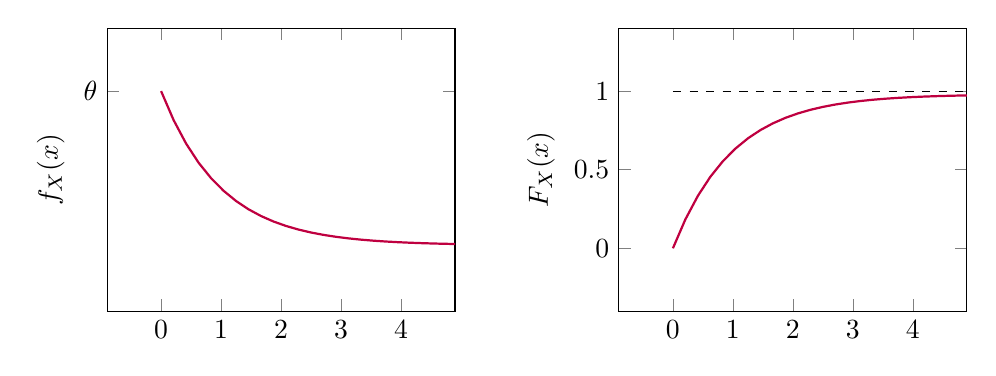
\begin{tikzpicture}
        \begin{axis}[
            width = 6cm,
            xmin = -0.9, xmax = 4.9,
            ymin = -0.4, ymax = 1.4,
            xtick distance = 1,
            ylabel = $f_X(x)$,
            ytick = {1},
            yticklabels = {$\theta$}
        ]
            \addplot[thick, purple, domain = 0:5] {0.02 + (0.98 * e^(-x))};
        \end{axis}
        
        \begin{axis}[
            width = 6cm,
            xmin = -0.9, xmax = 4.9,
            ymin = -0.4, ymax = 1.4,
            xtick distance = 1,
            ylabel = $F_X(x)$,
            ytick distance = 0.5,
            at = {(6.5cm, 0)}
        ]
            \addplot[thick, purple, domain = 0:5] {0.98 * (1 - e^(-x))};
            \draw[dashed] (axis cs: 0, 1) -- (axis cs: 5, 1);
        \end{axis}
    \end{tikzpicture}
\end{center}
\bigskip

Zmienna $X$ ma \textbf{rozkład normalny} (Gaussa) o wartości oczekiwanej $\mu$ i odchyleniu standardowym $\sigma$, oznaczany jako $\purple{X \sim \rpN(\mu, \sigma)}$, jeśli $X$ ma gęstość 
$$f_X(x) = \frac{1}{\sqrt{2\pi} \sigma} e^{-\frac{(x - \mu)^2}{2\sigma^2}}$$

Rozkład normalny ma dość skomplikowaną definicję. Suma dużej liczby niezależnych zmiennych, z których żadna nie dominuje pozostałych (tj. nie przyjmuje dużo większych wartości ani nie ma decydującego wpływu wynik) ma w przybliżeniu rozkład normalny. Przykładem może być wzrost lub masa człowieka o zbliżonych cechach, np. płci i rasie.

Rozkład $\rpN(0, 1)$ nazywamy \textbf{standardowym rozkładem normalnym}. Często pojawia się on w definicjach innych rozkładów oraz różnych rozumowaniach.

\begin{center}
    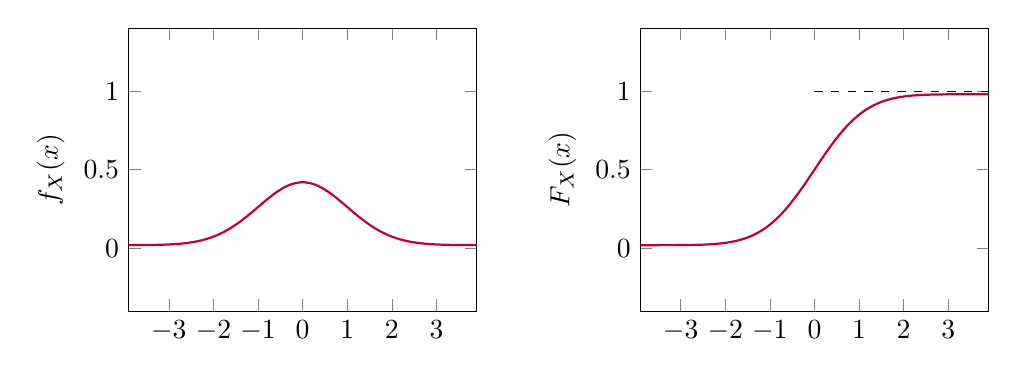
\begin{tikzpicture}
        \begin{axis}[
            width = 6cm,
            xmin = -3.9, xmax = 3.9,
            ymin = -0.4, ymax = 1.4,
            xtick distance = 1,
            ylabel = $f_X(x)$,
            ytick distance = 0.5,
            samples = 100
        ]
            \addplot[thick, purple] {0.02 + (0.4 * e^(-0.5 * x^2))};
        \end{axis}
        
        \begin{axis}[
            width = 6cm,
            xmin = -3.9, xmax = 3.9,
            ymin = -0.4, ymax = 1.4,
            xtick distance = 1,
            ylabel = $F_X(x)$,
            ytick distance = 0.5,
            samples = 100,
            at = {(6.5cm, 0)}
        ]
            \addplot[thick, purple] {0.02 + (0.48 * (1 + tanh(sqrt(pi)/2 * (x + 0.044715 * x^3))))};
            \draw[dashed] (axis cs: 0, 1) -- (axis cs: 5, 1);
        \end{axis}
    \end{tikzpicture}
\end{center}

Jeśli $X, Y$ są \purple{niezależnymi} zmiennymi losowymi o rozkładzie normalnym ze średnimi $\mu_X, \mu_Y$ oraz odchyleniami standardowymi $\sigma_X, \sigma_Y$, to
\begin{itemize}
    \item zmienna losowa $X + Y$ ma rozkład normalny $\rpN(\mu_X + \mu_Y, \sqrt{\sigma_X^2 + \sigma_Y^2})$,
    \item zmienna losowa $X - Y$ ma rozkład normalny $\rpN(\mu_X - \mu_Y, \sqrt{\sigma_X^2 + \sigma_Y^2})$.
\end{itemize}

\subsection{Parametry rozkładów ciągłych}

W ogólności \purple{wszystkie podstawowe własności wartości oczekiwanej i wariancji przenoszą się z przypadku dyskretnego na ciągły}. Dla formalności, poniżej uogólnimy jedynie podstawowe definicje.
\bigskip

Niech $X$ będzie ciągłą zmienną losową o gęstości $f_X$. \textbf{Wartością oczekiwaną} $X$ nazywamy wartość
$$\E X = \int_{-\infty}^{+\infty} x f_X(x) \dx,$$
o ile $|x|f_X(x)$ jest całkowalna. Jeśli wartość oczekiwana istnieje, to \textbf{wariancję} obliczamy ze standardowego wzoru:
$$\Var X = \E(X - \E X)^2 \textqq{albo} \Var X = \E(X^2) - (\E X)^2$$

\subsection{Wartości parametrów znanych rozkładów ciągłych}

Poniższa tabela przedstawia spis wartości oczekiwanych i wariancji dla znanych nam rozkładów ciągłych.

\begin{center}
\renewcommand{\arraystretch}{1.5}
\newcolumntype{C}{>{\centering\arraybackslash} m{3cm}}
\begin{tabular}{ C | C | C }
    & $\E X$ & $\Var X$ \\ \hline
    $X \sim \rpUnif(a, b)$ & $(a + b)/2$ & $(a - b)^2 / 12$ \\ \hline
    $X \sim \rpExp(\theta)$ & $1/\theta$ & $1/\theta^2$ \\ \hline
    $X \sim \rpN(\mu, \sigma)$ & $\mu$ & $\sigma$
\end{tabular}
\end{center}

\subsection{Centralne twierdzenie graniczne}

Rozkłady normalne należą do najważniejszych rozkładów w rachunku prawdopodobieństwa. Okazuje się, że wiele występujących w przyrodzie wielkości ma rozkład w przybliżeniu normalny, np. rozkład wzrostu, wagi, ilorazu inteligencji czy innych cech populacji. Matematyczne wyjaśnienie tego faktu opisuje \textbf{centralne twierdzenie graniczne}.
\bigskip

Niech $X_1, X_2 ...$ będzie ciągiem niezależnych zmiennych losowych o tym samym rozkładzie, wartości oczekiwanej $\mu$ i wariancji $\sigma^2 > 0$. Wówczas dla dowolnego $t \in \RR$ mamy
$$
\limn P\left(\frac{X_1 + X_2 + ... + X_n - n \mu}{\sigma \sqrt{n}} \leq t\right) = \Phi(t),
$$
gdzie $\Phi$ to dystrybuanta standardowego rozkładu normalnego $N(0,1)$. Jej konkretne wartości można znaleźć w tablicach matematycznych.

Twierdzenie to mówi, że rozkład sumy wielu niezależnych zmiennych o tym samym rozkładzie jest bliski normalnemu.

\begin{example}
    Rzucono monetą 10000 razy i okazało się, że orzeł wypadł 5200 razy. Sprawdzimy, jak duże są podstawy do przypuszczenia, że moneta jest niesymetryczna.

    Rozważmy ciąg zmiennych $X_i$ przyjmujących wartość 1, jeśli w $i$-tym rzucie wypadł orzeł, lub wartość 0 w przeciwnym przypadku. Jasne jest, że $X_1, X_2, ..., X_{10000}$ są niezależne o tym samym rozkładzie, możemy więc zastosować centralne twierdzenie graniczne, żeby oszacować prawdopodobieństwo rozważanego zdarzenia (5200 orłów w ciągu 10000 rzutów).

    Łatwo obliczamy $\E X_i = 1/2$ oraz $\Var X_i = 1/4$, stąd $\mu = 1/2$ i $\sigma = \sqrt{\Var X_i} = 1/2$ i dalej
    $$P(X_1 + X_2 + ... + X_{10000} \leq 5200) = P(X_1 + X_2 + ... + X_{10000} - 10000\mu \leq 5200 - 5000) =$$
    $$= P\left(\frac{X_1 + X_2 + ... + X_{10000} - 10000 \mu}{\sigma \sqrt{10000}} \leq \frac{200}{50}\right) \approx \Phi(4)$$

    Sprawdzając w tablicach: $\Phi(4) \approx 0.99997$, więc prawdopodobieństwo, że $X_1 + X_2 + ... + X_{10000} \geq 5200$ (zdarzenie przeciwne do obliczonego powyżej -- w 10000 rzutach monetą wyrzucimy przynajmniej 5200 orłów) ma prawdopodobieństwo $1 - \Phi(4) \approx 0.00003$. To bardzo mało; są więc podstawy, by sądzić, że moneta nie jest symetryczna.
\end{example}

\begin{problems}
    \prob Zmienne $X$ i $Y$ mają rozkład jednostajny na przedziale $[0, 2]$. Jeśli $Z = X + Y$, to
    \answers{$P(Z \geq 1) = \frac{7}{8}$}{$Z$ ma rozkład jednostajny na $[0, 4]$ i wartość oczekiwaną 2}{$P(|\mathrm{E}Z - Z| \geq 1) > \frac{2}{3}$}

    \prob Niech $F_{X}(t)$ będzie dystrybuantą pewnej zmiennej losowej $X$. Załóżmy, że $F_{X}(1)=\frac{1}{3}$. Wynika z tego, że
    \answers{istnieje takie $t$, że $F_{X}(t) = 1$}{$F_X(2) > \frac{1}{3}$}{istnieje takie $t$, że $F_{X}(t) < \frac{1}{4}$}

    \prob Niech $X$ i $Y$ będą niezależnymi zmiennymi losowymi. Wynika z tego, że
    \answers{jeśli $X$ i $Y$ mają rozkład Poissona, to $X - Y$ też}{jeśli $X$ i $Y$ mają rozkład normalny, to $X - Y$ też}{jeśli $X$ i $Y$ mają rozkład geometryczny, to $X - Y$ też}

    \prob Niech $X$ i $Y$ będą dwiema niezależnymi zmiennymi losowymi o rozkładzie normalnym o wartości oczekiwanej 0 i wariancji 4. Wynika z tego, że
    \answers
    {$X - Y$ ma taki sam rozkład jak $X + Y$}
    {odchylenie standardowe zmiennej losowej $X - Y$ jest równe 4}
    {dla $a, b > 0$ zmienna losowa $aX + bY$ ma rozkład normalny}
\end{problems}

\section{Łańcuchy Markowa}

% TODO
\begin{editorsnote}
    Rozdział nie jest jeszcze stworzony -- w historii przeanalizowanych na potrzeby tego repetytorium egzaminów nie pojawiło się żadne zadanie z łańcuchów Markowa.
\end{editorsnote}

\begin{solutions}
    % Kasia K
    \sol Istnieje przestrzeń probabilistyczna $\Omega$ i zdarzenia $A,B\subseteq\Omega$ takie, że $P(A)=P(B)=\frac{2}{3}$ oraz
    \answerss{$A$ i $B$ są niezależne}{$P(A|B)=\frac{1}{3}$}{$P(A|B)\neq P(B|A)$}{TAK}{NIE}{NIE}

    Przy rozwiązaniu tego typu zadań dobrze skorzystać z diagramu Venna. Łatwo można zauważyć, że zachodzi $\frac{1}{3} \leq P(A \cap B) \leq \frac{2}{3}$, a to pomoże w dalszych rozważaniach:
    \begin{enumerate}[\bf A.]
        \item Żeby $A$ i $B$ były niezależne, musi zachodzić
        $$P(A \cap B) = P(A) \cdot P(B) = \frac{4}{9}$$
        Ponieważ $\frac{1}{3} \leq \frac{4}{9} \leq \frac{2}{3}$, taka sytuacja jest możliwa.
        
        \item Tym razem mamy
        $$P(A | B) = \frac{P(A \cap B)}{P(B)} \wtw P(A \cap B) = P(A|B) \cdot P(B) = \frac{1}{3} \cdot \frac{2}{3} = \frac{2}{9}$$
        Ponieważ $\frac{2}{9} < \frac{1}{3}$, taka sytuacja nie może zajść.
        
        \item Zauważmy, że dla dowolnych zdarzeń $A, B$ spełniających warunki zadania jest
        $$P(A|B) = \frac{P(A \cap B)}{P(B)} = \frac{P(A \cap B)}{2/3} = \frac{P(A \cap B)}{P(A)} = P(B|A)$$
    \end{enumerate}

    %Tomek
    \sol Chcemy rozpalić ognisko, lecz mamy do dyspozycji tylko trzy zapałki. Prawdopodobieństwo rozpalenia ogniska pojedynczą zapałką wynosi $0.4$, dwiema złączonymi zapałkami -- $0.6$, zaś trzema złączonymi zapałkami -- $0.8$. Żeby zmaksymalizować prawdopodobieństwo rozpalenia ogniska, należy
    \answerss
    {użyć od razu trzech zapałek}
    {użyć najpierw dwóch zapałek, a potem jednej}
    {używać pojedynczych zapałek}
    {TAK}{NIE}{NIE}

    Oznaczmy zdarzenia:
    \begin{itemize}
        \item $A$ -- rozpalimy ognisko trzema złączonymi zapałkami,
        \item $B$ -- rozpalimy ognisko dwiema zapałkami, a potem jedną,
        \item $C$ -- rozpalimy ognisko trzema pojedynczymi zapałkami.
    \end{itemize}

    Obliczamy i porównujemy poszczególne prawdopodobieństwa:
    \begin{itemize}
        \item $P(A) = 0.8$
        \item $P(B) = 0.6 + (1 - 0.6) \cdot 0.4 = 0.76$ \gray{(odpalamy za pierwszym razem dwoma zapałkami lub nie odpalamy za pierwszym razem i odpalamy za drugim)}
        \item $P(C) = 0.4 + (1 - 0.4) \cdot 0.4 + (1 - 0.4)^2 \cdot 0.4 = 0.784$ \gray{(analogiczne rozumowanie -- rozpalamy za pierwszym, drugim albo trzecim razem)}
    \end{itemize}

    Najbardziej opłacalne jest więc użycie trzech złączonych zapałek.

    \sol Rzucamy 10 razy symetryczną monetą. Wynika z tego, że
    \answerss
    {prawdopodobieństwo, że wyrzucimy dokładnie 2 orły jest równe $\frac{45}{1024}$}
    {prawdopodobieństwo, że wyrzucimy orła w ostatnim rzucie pod warunkiem, że we wszystkich 10 rzutach wyrzucimy dokładnie 1 orła, jest równe $\frac{1}{2}$}
    {prawdopodobieństwo, że wyrzucimy orła w ostatnim rzucie pod warunkiem, że w pierwszych 9 rzutach wyrzucimy dokładnie 6 orłów, jest równe $\frac{1}{2}$}
    {TAK}{NIE}{NIE}

    \begin{enumerate}[\bf A.]
        \item Oznaczmy zdarzenie ,,wyrzucono dokładnie 2 orły'' jako $A$. W zadaniu mamy do czynienia ze schematem 10 prób Bernoulliego o prawdopodobieństwie sukcesu $\frac{1}{2}$ (wyrzucono orła). W związku z tym
        $$P(A) = \binom{10}{2} \left(\frac{1}{2}\right)^2 \left(1 - \frac{1}{2}\right)^8 = \frac{45}{2^{10}} = \frac{45}{1024}$$

        \item Wiedza o tym, że we wszystkich 10 rzutach wyrzuciliśmy dokładnie 1 orła, ogranicza nam przestrzeń zdarzeń elementarnych do 10 elementów: każdy z nich różni się pozycją orła. Tylko jedno zdarzenie elementarne posiada orła na ostatniej pozycji, więc szukane prawdopodobieństwo warunkowe wynosi $\frac{1}{10}$.

        \item Wiedza o tym, że w pierwszych 9 rzutach wyrzucimy dokładnie 6 orłów, nie dostarcza nam żadnych dodatkowych informacji na temat ostatniego rzutu -- jest on wykonywany niezależnie od pierwszych dziewięciu. W związku z tym w tak ograniczonej przestrzeni zdarzeń elementarnych jest tyle samo zdarzeń posiadających na ostatnim miejscu reszkę co zdarzeń na ostatnim miejscu z orłem. Prawdopodobieństwo wynosi więc $\frac{1}{2}$.

        Możemy również przekonać się o tym z obliczeń: oznaczmy zdarzenia
        \begin{itemize}
            \item $A$ -- wyrzucono orła w ostatnim rzucie,
            \item $B$ -- w pierwszych 9 rzutach wyrzucono dokładnie 6 orłów.
        \end{itemize}

        Zdarzenie $B$ to schemat 9 prób Bernoulliego o prawdopodobieństwie sukcesu $\frac{1}{2}$. Obliczamy kolejno:
        $$P(B) = \binom{9}{6} \left(\frac{1}{2}\right)^6 \left(1 - \frac{1}{2}\right)^3 = \frac{84}{2^{9}} = \frac{21}{128}$$
        $$P(A \cap B) = \frac{1}{2} \cdot P(B) = \frac{21}{256}$$
        $$P(A | B) = \frac{P(A \cap B)}{P(B)} = \frac{1}{2}$$
    \end{enumerate}

    % Julia
    \sol Mamy 9 ponumerowanych kart od 1 do 9. Dwie osoby $A$ oraz $B$ losują bez zwracania po jednej karcie. Wygrywa osoba, która wylosuje kartę z większym numerem. Prawdą jest, że
    \answerss{zdarzenia ,,wygrała osoba $A$'' oraz ,,osoba $A$ wylosowała kartę z numerem 5'' są niezależne}{zdarzenie ,,wygrała osoba $A$ pod warunkiem, że wylosowała kartę z numerem 7'' ma prawdopodobieństwo $\frac{3}{4}$}{zdarzenia ,,wygrała osoba $A$'' oraz ,,wygrała osoba $B$'' są niezależne}{TAK}{TAK}{NIE}

    Jasne jest, że $|\Omega| = 9 \cdot 8 = 72$.
    \begin{enumerate}[\bf A.]
        \item Oznaczmy zdarzenia $X$ -- wygrała osoba $A$, $Y$ -- osoba $A$ wylosowała kartę z numerem 5. Obliczamy:
        \begin{itemize}
            \item $P(X) = \frac{8 + 7 + ... + 1}{72} = \frac{1}{2}$ (zliczamy liczbę par $(a, b)$, w których $a > b$)
            \item $P(Y) = \frac{8}{72} = \frac{1}{9}$
            \item $P(X \cap Y) = \frac{4}{72} = \frac{1}{18}$
        \end{itemize}
        Ponieważ $P(X \cap Y) = P(X)P(Y)$, zdarzenia $X$ i $Y$ są niezależne.

        \item Oznaczmy zdarzenia $X$ -- wygrała osoba $A$, $Y$ -- osoba $A$ wylosowała kartę z numerem 7. Obliczamy:
        \begin{itemize}
            \item $P(X \cap Y) = \frac{6}{72} = \frac{1}{12}$
            \item $P(Y) = \frac{8}{72} = \frac{1}{9}$
            \item $P(X | Y) = \frac{P(X \cap Y)}{P(Y)} = \frac{3}{4}$
        \end{itemize}

        \item Oznaczmy zdarzenia $X$ -- wygrała osoba $A$, $Y$ -- wygrała osoba $B$. Obliczamy:
        \begin{itemize}
            \item $P(X) = P(Y) = \frac{1}{2}$
            \item $P(X \cap Y) = 0$
        \end{itemize}
        Ponieważ $P(X \cap Y) \neq P(X)P(Y)$, zdarzenia $X$ i $Y$ nie są niezależne.
    \end{enumerate}

    % Patryk
    \sol Rzucamy symetryczną kostką dwudziestościenną. Niech $X$ będzie liczbą wyrzuconych oczek. Wtedy niezależne są zdarzenia ,,wyrzucono parzystą liczbę oczek'' oraz
    \answerss
    {wyrzucono liczbę oczek podzielną przez $3$}
    {wyrzucono liczbę oczek podzielną przez $5$}
    {$X \leq 8$}
    {TAK}{TAK}{TAK}

    Łatwo rozwiążemy to zadanie za pomocą prostej intuicji idącej za niezależnością zdarzeń: ,,czy zajście zdarzenia $A$ daje dodatkową informację na temat zdarzenia $B$?''.
    
    Rozważmy, ile mamy liczb podzielnych przez 3 w kostce dwudziestościennej: $\{3, 6, 9, 12, 15, 18\}$, są więc 3 parzyste i 3 nieparzyste. Analogicznie dla liczb podzielnych przez 5: $\{5, 10, 15, 20\}$ -- 2 parzyste i 2 nieparzyste. Zdarzenie ,,wyrzucono parzystą liczbę oczek'' w żaden sposób nie dostarcza nam dodatkowych informacji o prawdopodobieństwie wyrzucenia liczby podzielnej przez 3 lub 5, bo jest tyle samo nieparzystych co parzystych wielokrotności tych liczb.
    
    To samo tyczy się prawdopodobieństwa wyrzucenia liczby mniejszej bądź równej 8: jest tyle samo parzystych i nieparzystych liczb w zbiorze $\{1, 2, ..., 8\}$, więc parzystość nie dostarcza nam żadnych dodatkowych informacji. 
    
    Wszystkie zdarzenia są więc niezależne. Można to łatwo potwierdzić za pomocą standardowych obliczeń (które tu pominiemy).

    % Patryk
    \sol Wrzucamy losowo dwie kule do dwóch urn. Wartość oczekiwana liczby niepustych urn jest równa
    \answerss
    {1}
    {$\frac{3}{2}$}
    {$2(1 - \frac{1}{e})$}
    {NIE}{TAK}{NIE}

    Oznaczmy przez $X$ liczbę niepustych urn. Zauważmy, że jedyne możliwe wartości $X$ to 1 i 2. Wartość ta jest jednoznacznie wyznaczona przez wrzucenie drugiej kuli -- albo trafi ona do tej samej urny, co pierwsza kula, albo do innej. Oba te zdarzenia są równie prawdopodobne (i niezależne od wrzucenia pierwszej kuli!), więc $P(X = 1) = P(X = 2) = \frac{1}{2}$. Mamy stąd
    $$\E X = 1 \cdot \frac{1}{2} + 2 \cdot \frac{1}{2} = \frac{3}{2}$$
    
    \sol Wrzucamy do worka $n \geq 3$ kul, każdą z nich malujemy niezależnie z prawdopodobieństwem $\frac{1}{2}$ na biało. Wartość oczekiwana liczby białych kul
    \answerss{wynosi $\frac{n(n-1)}{2}$}{wynosi $\frac{n}{2}$}{jest większa lub równa wariancji liczby białych kul}{NIE}{TAK}{TAK}

    Oznaczmy przez $X$ liczbę białych kul i podzielmy ją na $n$ niezależnych zmiennych $X_i$ równych 1, gdy $i$-ta kula jest biała, lub 0, gdy $i$-ta kula nie jest biała. Stąd $X = X_1 + X_2 + ... + X_n$.

    Mamy teraz
    $$\E X_i = 0 \cdot \frac{1}{2} + 1 \cdot \frac{1}{2} = \frac{1}{2}, \qquad \Var X_i = \E (X^2) - (\E X)^2 = \left(0^2 \cdot \frac{1}{2} + 1^2 \cdot \frac{1}{2}\right) - \frac{1}{4} = \frac{1}{4}$$
    i możemy skorzystać z liniowości wartości oczekiwanej oraz addytywności wariancji (ponieważ $X_i$ są niezależne):
    $$\E X = n \cdot \E X_i = \frac{n}{2}, \qquad \Var X = n \cdot \Var X_i = \frac{n}{4}$$

    % Jasiek
    \sol Dany jest generator bitów, dla którego każdy kolejny wygenerowany bit jest jedynką z prawdopodobieństwem 0.5. Niech $X$ będzie zmienną losową oznaczająca liczbę wygenerowanych jedynek przez ten generator w 100 próbach. Nie wiadomo, czy kolejne losowania są niezależne. Wówczas
    \answerss{$\mathrm{E}X = 50$}{$\mathrm{E}X = 50$, gdy kolejne bity są generowane niezależnie}{$\mathrm{Var}(X) = 25$}{TAK}{TAK}{NIE}

    Niech $X = X_1 + X_2 + ... + X_{100}$, gdzie $X_i$ jest równe $i$-temu wygenerowanemu bitowi. Mamy
    $$\E X_i = 0 \cdot \frac{1}{2} + 1 \cdot \frac{1}{2} = \frac{1}{2}, \qquad \Var X_i = \E (X^2) - (\E X)^2 = \left(0^2 \cdot \frac{1}{2} + 1^2 \cdot \frac{1}{2}\right) - \frac{1}{4} = \frac{1}{4}$$

    Prawdziwość podpunktów \textbf{A.} i \textbf{B.} wynika wprost z liniowości wartości oczekiwanej -- nie ma tu znaczenia, czy losowania kolejnych bitów są niezależne. W obu przypadkach $\E X = 100 \cdot \E X_i = 50$.

    Żeby wariancja $X$ była równa 25, musiałoby być $\Var X = 100 \cdot \Var X_i = 25$, ale to jest prawdziwe wyłącznie, gdy zmienne $X_i$ są ze sobą niezależne (wynika to wprost z addytywności wariancji). W związku z tym podpunkt \textbf{C.} jest fałszywy.
    
    \sol Niech $X$ i $Y$ to zmienne losowe, takie że $\E X = 1$, $\Var X = 4$ i $Y = 2X + 3$. Wtedy
    \answerss{$\E Y = 4$}{$\sigma(Y) = 4$}{$\Var Y = 4$}
    {NIE}{TAK}{NIE}

    Z liniowości wartości oczekiwanej mamy, że $\E Y = 2 \cdot \E X + \E 3 = 2 \cdot 1 + 3 = 5$, co dowodzi fałszywości podpunktu \textbf{A.}

    Skorzystamy z własności wartości oczekiwanej, że jeśli $X$ jest zmienną losową o skończonej wartości oczekiwanej oraz $a, b$ są liczbami rzeczywistymi, to $\Var (aX + b) = a^2 \Var X$. U nas
    $$\Var Y = \Var (2X + 3) = 2^2 \Var X = 16 \textqq{ i tym samym } \sigma(Y) = \sqrt{\Var Y} = 4$$

    Stąd podpunkt \textbf{B.} jest prawdziwy i \textbf{C.} jest fałszywy.

    \sol Niech $X$ i $Y$ będą zdarzeniami niezależnymi, wtedy
    \answerss
    {$\mathrm{E}(X - Y) = \mathrm{E}X - \mathrm{E}Y$}
    {$\mathrm{E}(XY) = \mathrm{E}X \cdot \mathrm{E}Y$}
    {$\mathrm{E}(X / Y) = \mathrm{E}X / \mathrm{E}Y$}
    {TAK}{TAK}{NIE}

    Podpunkty \textbf{A.} i \textbf{B.} są prawdziwe, odpowiednio z własności liniowości i multiplikatywności wartości oczekiwanej.

    Nietrudno też zauważyć, że jeśli $\E Y = 0$, równość w podpunkcie \textbf{C.} nie zachodzi.

    % Grześ + Jasiek
    \sol Niech $X$ i $Y$ będą zmiennymi losowymi o wartościach nieujemnych. Wynika z tego, że
    \answerss{$\mathrm{E}(XY)=\mathrm{E}X\cdot \mathrm{E}Y$, jeśli $X$ i $Y$ są niezależne}{$\mathrm{E}(\min(X,Y))=\min(\mathrm{E}X,\mathrm{E}Y)$}{$\mathrm{E}(\min(X,Y))=\min(\mathrm{E}X,\mathrm{E}Y)$, jeśli $X$ i $Y$ są niezależne}{TAK}{NIE}{NIE}

    Podpunkt \textbf{A.} jest prawdziwy, wprost z definicji multiplikatywności wartości oczekiwanej.

    Do pokazania kontrprzykładu do \textbf{C.} (a przy okazji do \textbf{B.}) rozważmy dwukrotny rzut kostką oraz oznaczmy przez $X$ i $Y$ uzyskane wyniki przy odpowiednio pierwszym i drugim rzucie (zmienne te są w oczywisty sposób niezależne). Wtedy $\E X = \E Y = 3.5$, czyli $\min(\E X, \E Y) = 3.5$.
    
    Obliczymy teraz $\E (\min(X, Y))$. Jest to wartość oczekiwana mniejszej z wyrzuconych wartości. Mamy 11 opcji, że będzie to liczba 1:
    $$\big(\{6, 1\}, \{5, 1\}, ..., \{1, 1\}, \{1, 2\}, ..., \{1, 6\}\big)$$
    Analogicznie sprawdzamy, że jest 9 opcji, że będzie to liczba 2, itd. Zatem
    $$
    \E \big(\min(X, Y)\big) = \frac{1}{36} (11 \cdot 1 + 9 \cdot 2 + 7 \cdot 3 + 5 \cdot 4 + 3 \cdot 5 + 1 \cdot 6) \approx 2.53 \neq 3.5
    $$
    
    \sol Niech $X$ będzie zmienną losową reprezentującą długość trwania programu dla różnych wejść, niech $\mu$ to wartość oczekiwana $X$, zaś $\sigma$ to odchylenie standardowe. Prawdą jest, że
    \answerss{$P(X > 2\mu) \leq \frac{1}{4}$}{$P(X > \mu + 2\sigma) \leq \frac{1}{4}$}{$P(X > 100\mu) \leq \frac{1}{10^{10}}$}{NIE}{TAK}{NIE}

    \begin{enumerate}[\bf A.]
        \item Wstawiając $c = 2\mu$ do nierówności Markowa, otrzymujemy
        $$P(X \geq 2 \mu) \leq \frac{\mu}{2\mu} = \frac{1}{2},$$
        co pozwala nam podejrzewać, że odpowiedź jest fałszywa. Rzeczywiście, nietrudno o kontrprzykład: niech $P(X = 2.01) = P(X = 0.49) = P(X = 0.5) = \frac{1}{3}$. Widzimy, że $\E X = 1$, ale
        $$P(X > 2\mu) = P(X > 2) = \frac{1}{3} > \frac{1}{4}$$

        \item Skorzystamy z nierówności Czebyszewa. Biorąc $c = 2\sigma$ mamy
        $$P(|X - \mu| \geq 2 \sigma) \leq \frac{\sigma^2}{(2 \sigma)^2} = \frac{1}{4}$$
        Zauważmy, że
        $$P(|X - \mu| \geq 2 \sigma) = P(X \geq \mu + 2 \sigma) + P(X \leq \mu - 2 \sigma) \leq \frac{1}{4},$$
        więc w szczególności $P(X \geq \mu + 2 \sigma) \leq \frac{1}{4}$ i odpowiedź jest prawdziwa.

        \item Nierówność Markowa jest w tym przypadku zbyt słaba (jej ograniczenie z góry jest znacząco za małe), a inne znane nam nierówności nie pozwalają nam uzyskać lepszego wyniku. Taka sytuacja sugeruje fałszywość nierówności, co pokażemy poprzez poniższy kontrprzykład.

        Weżmy $P(X = 101) = \frac{1}{102}$ oraz $P(X = \frac{1}{101}) = \frac{101}{102}$. W oczywisty sposób $\E X = 1$, ale
        $$P(X > 100\mu) = P(X > 100) = \frac{1}{102} > \frac{1}{10^{10}}$$
    \end{enumerate}

    \sol Zmienne $X$ i $Y$ mają rozkład jednostajny na przedziale $[0, 2]$. Jeśli $Z = X + Y$, to
    \answerss{$P(Z \geq 1) = \frac{7}{8}$}{$Z$ ma rozkład jednostajny na $[0, 4]$ i wartość oczekiwaną 2}{$P(|\mathrm{E}Z - Z| \geq 1) > \frac{2}{3}$}{TAK}{NIE}{NIE}

    \begin{enumerate}[\bf A.]
        \item Ponieważ zmienne $X, Y$ mają rozkład jednostajny, wykorzystamy prawdopodobieństwo geometryczne. Zaznaczmy w układzie współrzędnych zdarzenie $X + Y \geq 1$:

        \begin{center}
        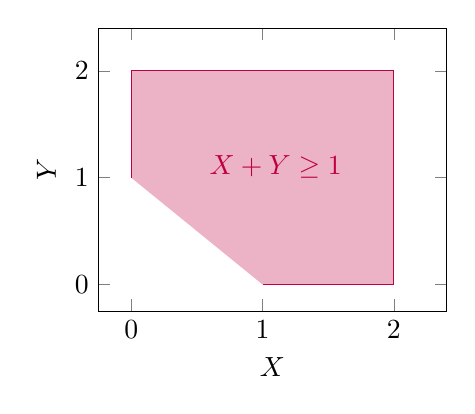
\begin{tikzpicture}
            \begin{axis}[
                width = 6 cm,
                xmin = -0.25, xmax = 2.4,
                ymin = -0.25, ymax = 2.4,
                xlabel = $X$,
                xtick distance = 1,
                ylabel = $Y$,
                ytick distance = 1,
            ]                
                \addplot [
                    draw=purple,
                    fill=purple,
                    fill opacity=0.3,
                ] coordinates {(0, 1) (0, 2) (2, 2) (2, 0) (1, 0)};                
                \node at (axis cs: 1.1, 1.1) {\textcolor{purple}{$X + Y \geq 1$}};
            \end{axis}
        \end{tikzpicture}
        \end{center}

        Widzimy, że szukane zdarzenie zajmuje dokładnie $\frac{7}{8}$ całego kwadratu $2 \times 2$. Odpowiedź jest więc prawdziwa.

        \item $Z$ nie ma rozkładu jednostajnego, intuicyjnie widać, że np. częściej wypadnie wynik 2 niż 0. Żeby się o tym przekonać, możemy obliczyć funkcję gęstości $Z$. Użyjemy znanego nam wzoru na gęstość zmiennej będącej sumą dwóch niezależnych zmiennych losowych:
        $$f_Z(x) = \int_{-\infty}^{+\infty} f_X(y) f_Y(x - y) \dy$$

        Gęstości $f_X, f_Y$ są takie same i, z definicji rozkładu jednostajnego, są dane wzorem
        $$
        f_X(x) = \begin{cases} 
            \frac{1}{2} & \text{dla } x \in [0, 2], \\
            0 & \text{wpp.}
        \end{cases}
        $$

        Ponieważ $f_X, f_Y$ są niezerowe wyłącznie w przedziale $[0, 2]$, ograniczymy całkowanie do tego przedziału. Obliczamy:
        \begin{itemize}
            \item dla $f_X(y) \neq 0$, czyli $x \in [0, 2]$:
            $$f_Z(x) = \int_{0}^{x} f_X(y) f_Y(x - y) \dy = \int_{0}^{x} \frac{1}{2} \cdot \frac{1}{2} \dy = \frac{1}{4} \int_{0}^{x} \dy = \frac{1}{4} \cdot y \big|_0^x = \frac{x}{4}$$

            \item dla $f_Y(x - y) \neq 0$, czyli $x \in [2, 4]$:
            $$f_Z(x) = \int_{x - 2}^{2} f_X(y) f_Y(x - y) \dy = \int_{x - 2}^{2} \frac{1}{2} \cdot \frac{1}{2} \dy = \frac{1}{4} \int_{x - 2}^{2} \dy = \frac{1}{4} \cdot y \big|_{x - 2}^2 = \frac{1}{4}\big(2 - (x - 2)\big) = 1 - \frac{x}{4}$$
        \end{itemize}

        Ostatecznie funkcją gęstości $Z$ jest więc
        $$
        f_Z(x) = \begin{cases}
            \frac{x}{4} & \text{dla } x \in [0, 2), \\
            1 - \frac{x}{4} & \text{dla } x \in [2, 4], \\
            0 & \text{wpp.}
        \end{cases}
        $$
        i pokazuje to, że $Z$ nie ma rozkładu jednostajnego.

        \item Z nierówności Czebyszewa mamy, że $P(|\E Z - Z| \geq 1) \leq \Var Z$. Nietrudno pokazać, że wariancja $Z$ jest równa $\frac{2}{3}$: ze wzoru na wariancję rozkładu jednostajnego $\rpUnif(0, 2)$ mamy
        $$\Var X = \Var Y = \frac{(2 - 0)^2}{12} = \frac{1}{3},$$
        a skoro $Z$ jest sumą dwóch niezależnych zmiennych, możemy skorzystać z addytywności wariancji:
        $$\Var Z = \Var X + \Var Y = \frac{2}{3}$$
    \end{enumerate}

    % Grześ + Jasiek
    \sol Niech $F_{X}(t)$ będzie dystrybuantą pewnej zmiennej losowej $X$. Załóżmy, że $F_{X}(1)=\frac{1}{3}$. Wynika z tego, że
    \answerss{istnieje takie $t$, że $F_{X}(t) = 1$}{$F_X(2) > \frac{1}{3}$}{istnieje takie $t$, że $F_{X}(t) < \frac{1}{4}$}{NIE}{NIE}{TAK}

    \begin{enumerate}[\bf A.]
        \item Zgodnie z własnościami dystrybuanty, mamy pewność, że $\Lim_{x \to \infty} F_X(x) = 1$, ale to niekoniecznie oznacza, że dla pewnego argumentu wartość 1 jest osiągana. Istotnie, nietrudno o przykład, w którym prosta $y = 1$ jest asymptotą poziomą; dzieje się tak choćby dla standardowego rozkładu normalnego:

        \begin{center}
            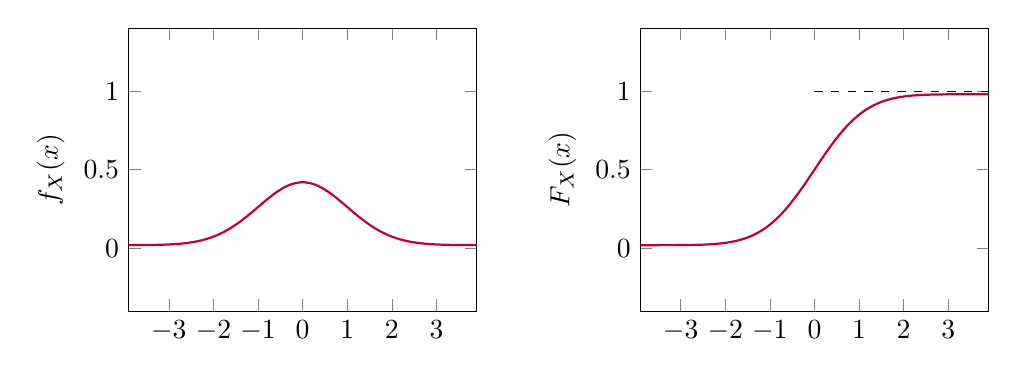
\begin{tikzpicture}
                \begin{axis}[
                    width = 6cm,
                    xmin = -3.9, xmax = 3.9,
                    ymin = -0.4, ymax = 1.4,
                    xtick distance = 1,
                    ylabel = $f_X(x)$,
                    ytick distance = 0.5,
                    samples = 100
                ]
                    \addplot[thick, purple] {0.02 + (0.4 * e^(-0.5 * x^2))};
                \end{axis}
                
                \begin{axis}[
                    width = 6cm,
                    xmin = -3.9, xmax = 3.9,
                    ymin = -0.4, ymax = 1.4,
                    xtick distance = 1,
                    ylabel = $F_X(x)$,
                    ytick distance = 0.5,
                    samples = 100,
                    at = {(6.5cm, 0)}
                ]
                    \addplot[thick, purple] {0.02 + (0.48 * (1 + tanh(sqrt(pi)/2 * (x + 0.044715 * x^3))))};
                    \draw[dashed] (axis cs: 0, 1) -- (axis cs: 5, 1);
                \end{axis}
            \end{tikzpicture}
        \end{center}

        Wówczas nie istnieje żadne $t \in \RR$, dla którego $F_X(t) = 1$.

        \item Dystrybuanta jest funkcją niemalejącą, co oznacza, że $F_X(2) \geq \frac{1}{3}$. Może więc być $F_X(2) = \frac{1}{3}$, co pokazuje fałszywość odpowiedzi.

        \item Ponieważ $\Lim_{x \to -\infty} F_X(x) = 0$, dla bardzo małych argumentów będziemy uzyskiwali bardzo małe wartości, na pewno mniejsze od $\frac{1}{4}$.
    \end{enumerate}

    \sol Niech $X$ i $Y$ będą niezależnymi zmiennymi losowymi. Wynika z tego, że
    \answerss{jeśli $X$ i $Y$ mają rozkład Poissona, to $X - Y$ też}{jeśli $X$ i $Y$ mają rozkład normalny, to $X - Y$ też}{jeśli $X$ i $Y$ mają rozkład geometryczny, to $X - Y$ też}{NIE}{TAK}{NIE}

    \begin{enumerate}[\bf A.]
        \item Niech $X \sim \rpPois(\lambda_X)$ oraz $Y \sim \rpPois(\lambda_Y)$. Takie zmienne modelują liczbę wystąpień pewnego nieprzewidywalnego zdarzenia w ustalonym przedziale czasu, przy czym zdarzenia te mają średnią częstość wystąpienia odpowiednio $\lambda_X, \lambda_Y$.

        O ile zmienna $X + Y$ ma rozkład Poissona (badamy łączne wystąpienia obu niezależnych zdarzeń) z parametrem $\lambda_X + \lambda_Y$, o tyle $X - Y$ napotyka na problem: zmienne o rozkładzie Poissona przyjmują wartości całkowite nieujemne, podczas gdy różnica $\lambda_X - \lambda_Y$ może potencjalnie przyjąć wartości mniejsze od 0.

        \item Zgodnie ze znanym nam faktem, różnica dwóch niezależnych zmiennych losowych o rozkładach normalnych odpowiednio $\rpN(\mu_X, \sigma_X)$ oraz $\rpN(\mu_Y, \sigma_Y)$ ma również rozkład normalny z wartością oczekiwaną $\mu_X - \mu_Y$ i odchyleniem standardowym $\sqrt{\sigma_X^2 + \sigma_Y^2}$.

        \item Kontrargument jest bardzo podobny jak w podpunkcie \textbf{A.} Zmienna o rozkładzie geometrycznym może przyjmować wyłącznie wartości całkowite dodatnie, a różnica $X - Y$ potencjalnie przyjmie wartość ujemną bądź zerową.
    \end{enumerate}

    \sol Niech $X$ i $Y$ będą dwiema niezależnymi zmiennymi losowymi o rozkładzie normalnym o wartości oczekiwanej 0 i wariancji 4. Wynika z tego, że
    \answerss
    {$X - Y$ ma taki sam rozkład jak $X + Y$}
    {odchylenie standardowe zmiennej losowej $X - Y$ jest równe 4}
    {dla $a, b > 0$ zmienna losowa $aX + bY$ ma rozkład normalny}
    {TAK}{NIE}{TAK}

    \begin{enumerate}[\bf A.]
        \item Korzystając ze znanych nam faktów na temat rozkładu sumy i różnicy dwóch niezależnych zmiennych losowych o rozkładzie normalnym otrzymujemy:
        $$X - Y \sim \rpN(\mu_X - \mu_Y, \sqrt{\sigma_X^2 + \sigma_Y^2}) \sim \rpN(0, \sqrt{8})$$
        $$X + Y \sim \rpN(\mu_X + \mu_Y, \sqrt{\sigma_X^2 + \sigma_Y^2}) \sim \rpN(0, \sqrt{8})$$

        \item Jak pokazaliśmy w podpunkcie \textbf{A.}, odchylenie standardowe zmiennej $X - Y$ jest równe $\sqrt{8}$.

        \item Nietrudno intuicyjnie zauważyć, że zmienne $aX, bY$ mają rozkład normalny o przeskalowanych wartościach względem $X$ i $Y$. Ponieważ suma niezależnych zmiennych o rozkładzie normalnym ma również rozkład normalny, odpowiedź jest prawdziwa.
    \end{enumerate}
\end{solutions}

